\PassOptionsToPackage{hyphens}{url}
\documentclass[conference]{IEEEtran}
\IEEEoverridecommandlockouts
\usepackage{cite}
\usepackage{amsmath,amssymb}
\usepackage{graphicx}
\usepackage{booktabs}
\usepackage{multirow}
\usepackage{array}
\usepackage{url}
\usepackage{xcolor}
\usepackage{tikz}
\usetikzlibrary{positioning,arrows.meta}
\usepackage[hidelinks]{hyperref}

% numbers.tex and every tab_*.tex are generated by paper/experiment/citebench/make_tex.py (never edited by hand);
% numbers_case.tex is generated by case_study/make_case_tex.mjs from the worked-case results.
\newcommand{\AuditCorrect}{92}
\newcommand{\AuditMisCorrect}{4}
\newcommand{\AuditMisN}{4}
\newcommand{\AuditN}{95}
\newcommand{\AuditNFCorrect}{38}
\newcommand{\AuditNFFab}{27}
\newcommand{\AuditNFGeneric}{9}
\newcommand{\AuditNFMisdated}{1}
\newcommand{\AuditNFMiss}{2}
\newcommand{\AuditNFN}{40}
\newcommand{\AuditNFNotJudgment}{1}
\newcommand{\AuditPct}{96.8\%}
\newcommand{\AuditVerCorrect}{39}
\newcommand{\AuditVerN}{40}
\newcommand{\AuditWYCorrect}{11}
\newcommand{\AuditWYN}{11}
\newcommand{\BestTOneCorrect}{1}
\newcommand{\CasesAllClosed}{450}
\newcommand{\CasesAllFeedback}{235}
\newcommand{\CasesAllName}{399}
\newcommand{\CasesAllTopic}{466}
\newcommand{\CasesAllTopicPrior}{463}
\newcommand{\CasesClosedAll}{450}
\newcommand{\CasesClosedGemma}{117}
\newcommand{\CasesClosedLlama}{114}
\newcommand{\CasesClosedQwen}{117}
\newcommand{\CasesClosedQwenVL}{102}
\newcommand{\CasesFeedbackGemma}{46}
\newcommand{\CasesFeedbackLlama}{75}
\newcommand{\CasesFeedbackQwen}{60}
\newcommand{\CasesFeedbackQwenVL}{54}
\newcommand{\CasesSearchAll}{399}
\newcommand{\CasesSearchGemma}{108}
\newcommand{\CasesSearchLlama}{95}
\newcommand{\CasesSearchQwen}{97}
\newcommand{\CasesSearchQwenVL}{99}
\newcommand{\CasesTopicGemma}{120}
\newcommand{\CasesTopicLlama}{115}
\newcommand{\CasesTopicPriorGemma}{117}
\newcommand{\CasesTopicPriorLlama}{111}
\newcommand{\CasesTopicPriorQwen}{116}
\newcommand{\CasesTopicPriorQwenVL}{119}
\newcommand{\CasesTopicQwen}{112}
\newcommand{\CasesTopicQwenVL}{119}
\newcommand{\CollideDiffBothPct}{88.3\%}
\newcommand{\CollideLost}{62{,}006}
\newcommand{\CollideRows}{123{,}131}
\newcommand{\CollideStems}{61{,}125}
\newcommand{\CorpusCourts}{26}
\newcommand{\CorpusHC}{19{,}281{,}597}
\newcommand{\CorpusSC}{38{,}366}
\newcommand{\CorpusTotal}{19{,}319{,}963}
\newcommand{\CorpusYearMax}{2026}
\newcommand{\CorpusYearMin}{1950}
\newcommand{\DistinctAnswersGemma}{26}
\newcommand{\DistinctAnswersLlama}{40}
\newcommand{\DistinctAnswersQwen}{0}
\newcommand{\DistinctAnswersQwenThink}{23}
\newcommand{\DistinctAnswersQwenVL}{0}
\newcommand{\EmbedRate}{8}
\newcommand{\GraphAgreeN}{70{,}235}
\newcommand{\GraphAgreePct}{68.9\%}
\newcommand{\GraphCheckN}{60}
\newcommand{\GraphCheckOK}{60}
\newcommand{\GraphCheckPct}{100.0\%}
\newcommand{\GraphCited}{21{,}518}
\newcommand{\GraphCitedPct}{56.1\%}
\newcommand{\GraphCiting}{22{,}483}
\newcommand{\GraphConflict}{749}
\newcommand{\GraphEdges}{109{,}370}
\newcommand{\GraphExact}{68{,}523}
\newcommand{\GraphJudgments}{28{,}253}
\newcommand{\GraphKindAIR}{25{,}976}
\newcommand{\GraphKindAIRPct}{54.3\%}
\newcommand{\GraphKindINSC}{3{,}237}
\newcommand{\GraphKindINSCPct}{27.8\%}
\newcommand{\GraphKindSCC}{105{,}106}
\newcommand{\GraphKindSCCPct}{66.5\%}
\newcommand{\GraphKindSCR}{86{,}443}
\newcommand{\GraphKindSCRPct}{79.2\%}
\newcommand{\GraphLandmarkCited}{50}
\newcommand{\GraphLandmarkN}{51}
\newcommand{\GraphLandmarkPct}{98.9}
\newcommand{\GraphLater}{53}
\newcommand{\GraphLaterPct}{0.05\%}
\newcommand{\GraphLaterPctExact}{0.04\%}
\newcommand{\GraphLaterPctName}{0.06\%}
\newcommand{\GraphLaterPctParallel}{0.00\%}
\newcommand{\GraphMaxIn}{261}
\newcommand{\GraphMedianOut}{3}
\newcommand{\GraphName}{44{,}846}
\newcommand{\GraphNamePrecN}{46{,}091}
\newcommand{\GraphNamePrecOK}{45{,}342}
\newcommand{\GraphNamePrecPct}{98.4\%}
\newcommand{\GraphParallel}{40{,}013}
\newcommand{\GraphResolved}{153{,}382}
\newcommand{\GraphResolvedPct}{75.2\%}
\newcommand{\GraphTextFail}{9}
\newcommand{\GraphTextOK}{38{,}357}
\newcommand{\GraphTopFiveN}{141}
\newcommand{\GraphTopFourN}{150}
\newcommand{\GraphTopOneN}{261}
\newcommand{\GraphTopThreeN}{155}
\newcommand{\GraphTopTwoN}{170}
\newcommand{\GraphUnits}{203{,}915}
\newcommand{\INSCCompleteCount}{61}
\newcommand{\INSCCovMax}{79\%}
\newcommand{\INSCCovMin}{17\%}
\newcommand{\INSCIncompleteList}{1961, 1994 and 1997}
\newcommand{\LatBenchDate}{2026-09-30}
\newcommand{\LatCommonFirstMax}{8{,}750}
\newcommand{\LatCommonFirstMedian}{2{,}826}
\newcommand{\LatCommonWarmMedian}{270}
\newcommand{\LatExactMax}{15}
\newcommand{\LatExactMedian}{2.0}
\newcommand{\LatFallbackFirst}{0}
\newcommand{\LatFallbackWarm}{0}
\newcommand{\LatQueries}{129}
\newcommand{\LinkedPct}{99.1\%}
\newcommand{\MPLinked}{5}
\newcommand{\MPMobile}{42{,}695}
\newcommand{\MaxWrongLenientGemma}{0.34}
\newcommand{\MaxWrongLenientLlama}{0.36}
\newcommand{\MaxWrongLenientQwen}{--}
\newcommand{\MaxWrongLenientQwenThink}{0.19}
\newcommand{\MaxWrongLenientQwenVL}{--}
\newcommand{\MisTopicGemma}{2}
\newcommand{\MisTopicLlama}{0}
\newcommand{\MisTopicPriorGemma}{2}
\newcommand{\MisTopicPriorLlama}{1}
\newcommand{\MisTopicPriorQwen}{1}
\newcommand{\MisTopicPriorQwenVL}{2}
\newcommand{\MisTopicQwen}{3}
\newcommand{\MisTopicQwenVL}{2}
\newcommand{\MobileLinked}{1{,}122{,}387}
\newcommand{\MobileLinkedPct}{86.9\%}
\newcommand{\MobilePct}{6.7\%}
\newcommand{\MobileRecentPct}{97.8\%}
\newcommand{\MobileTotal}{1{,}291{,}516}
\newcommand{\MobileUnrecov}{169{,}129}
\newcommand{\NFAllClosed}{239}
\newcommand{\NFAllFeedback}{52}
\newcommand{\NFAllName}{8}
\newcommand{\NFAllTopic}{2}
\newcommand{\NFAllTopicPrior}{1}
\newcommand{\NFClosedAll}{239}
\newcommand{\NFClosedGemma}{81}
\newcommand{\NFClosedLlama}{42}
\newcommand{\NFClosedQwen}{49}
\newcommand{\NFClosedQwenVL}{67}
\newcommand{\NFFeedbackGemma}{16}
\newcommand{\NFFeedbackLlama}{4}
\newcommand{\NFFeedbackQwen}{1}
\newcommand{\NFFeedbackQwenVL}{31}
\newcommand{\NFSearchAll}{8}
\newcommand{\NFSearchGemma}{1}
\newcommand{\NFSearchLlama}{4}
\newcommand{\NFSearchQwen}{1}
\newcommand{\NFSearchQwenVL}{2}
\newcommand{\NFTopicGemma}{0}
\newcommand{\NFTopicLlama}{2}
\newcommand{\NFTopicPriorGemma}{0}
\newcommand{\NFTopicPriorLlama}{1}
\newcommand{\NFTopicPriorQwen}{0}
\newcommand{\NFTopicPriorQwenVL}{0}
\newcommand{\NFTopicQwen}{0}
\newcommand{\NFTopicQwenVL}{0}
\newcommand{\NoLink}{169{,}129}
\newcommand{\NoThinkMedianSec}{0.5}
\newcommand{\NoThinkTFourNFPct}{41.9\%}
\newcommand{\NoThinkTFourVerPct}{50.4\%}
\newcommand{\NonmobileChecked}{454}
\newcommand{\NonmobileCourts}{24}
\newcommand{\NumItems}{403}
\newcommand{\NumJudgments}{101}
\newcommand{\NumLandmark}{51}
\newcommand{\NumModels}{four}
\newcommand{\NumRandom}{50}
\newcommand{\NumRefJudgments}{70}
\newcommand{\NumTOne}{202}
\newcommand{\NumTThree}{101}
\newcommand{\NumTTwo}{60}
\newcommand{\NumTopics}{40}
\newcommand{\PairClosedTopicGained}{79}
\newcommand{\PairClosedTopicLost}{18}
\newcommand{\PairClosedTopicP}{$<$0.001}
\newcommand{\PairClosedTopicPriorGained}{96}
\newcommand{\PairClosedTopicPriorLost}{11}
\newcommand{\PairClosedTopicPriorP}{$<$0.001}
\newcommand{\PairTopicTopicPriorGained}{27}
\newcommand{\PairTopicTopicPriorLost}{3}
\newcommand{\PairTopicTopicPriorP}{$<$0.001}
\newcommand{\PairsChecked}{60}
\newcommand{\PairsDiffer}{60}
\newcommand{\PilotN}{502}
\newcommand{\QBmHitFive}{28}
\newcommand{\QBmHitTen}{30}
\newcommand{\QBmHitThree}{25}
\newcommand{\QBmRTen}{0.63}
\newcommand{\QDenseHitFive}{31}
\newcommand{\QDenseHitTen}{35}
\newcommand{\QDenseHitThree}{29}
\newcommand{\QDensePriorHitFive}{36}
\newcommand{\QDensePriorHitTen}{38}
\newcommand{\QDensePriorHitThree}{34}
\newcommand{\QDensePriorRTen}{0.84}
\newcommand{\QDenseRTen}{0.76}
\newcommand{\QHybridHitFive}{30}
\newcommand{\QHybridHitTen}{36}
\newcommand{\QHybridHitThree}{28}
\newcommand{\QHybridPriorHitFive}{35}
\newcommand{\QHybridPriorHitTen}{37}
\newcommand{\QHybridPriorHitThree}{33}
\newcommand{\QHybridPriorRTen}{0.84}
\newcommand{\QHybridRTen}{0.77}
\newcommand{\QPopHitFive}{2}
\newcommand{\QPopHitTen}{2}
\newcommand{\QPopHitThree}{2}
\newcommand{\QPopRTen}{0.04}
\newcommand{\QueryMs}{84}
\newcommand{\RecBmHitTen}{66.2\%}
\newcommand{\RecBmMRR}{0.390}
\newcommand{\RecBmPriorHitTen}{74.0\%}
\newcommand{\RecBmPriorMRR}{0.455}
\newcommand{\RecBmPriorRFifty}{0.381}
\newcommand{\RecBmPriorRTen}{0.182}
\newcommand{\RecBmPriorRTenCI}{0.172--0.193}
\newcommand{\RecBmRFifty}{0.321}
\newcommand{\RecBmRTen}{0.151}
\newcommand{\RecBmRTenCI}{0.142--0.162}
\newcommand{\RecDenseHitTen}{61.4\%}
\newcommand{\RecDenseMRR}{0.362}
\newcommand{\RecDensePriorHitTen}{68.6\%}
\newcommand{\RecDensePriorMRR}{0.426}
\newcommand{\RecDensePriorRFifty}{0.323}
\newcommand{\RecDensePriorRTen}{0.159}
\newcommand{\RecDensePriorRTenCI}{0.148--0.170}
\newcommand{\RecDenseRFifty}{0.286}
\newcommand{\RecDenseRTen}{0.136}
\newcommand{\RecDenseRTenCI}{0.126--0.146}
\newcommand{\RecDiffHybrid}{$+$0.016}
\newcommand{\RecDiffHybridBetter}{213}
\newcommand{\RecDiffHybridCI}{$+$0.011 to $+$0.021}
\newcommand{\RecDiffHybridWorse}{118}
\newcommand{\RecDiffPrior}{$+$0.036}
\newcommand{\RecDiffPriorBetter}{350}
\newcommand{\RecDiffPriorBm}{$+$0.031}
\newcommand{\RecDiffPriorBmBetter}{299}
\newcommand{\RecDiffPriorBmCI}{$+$0.025 to $+$0.036}
\newcommand{\RecDiffPriorBmWorse}{79}
\newcommand{\RecDiffPriorCI}{$+$0.030 to $+$0.043}
\newcommand{\RecDiffPriorDense}{$+$0.022}
\newcommand{\RecDiffPriorDenseBetter}{303}
\newcommand{\RecDiffPriorDenseCI}{$+$0.016 to $+$0.029}
\newcommand{\RecDiffPriorDenseWorse}{144}
\newcommand{\RecDiffPriorWorse}{99}
\newcommand{\RecHybridHitTen}{68.9\%}
\newcommand{\RecHybridMRR}{0.420}
\newcommand{\RecHybridPriorHitTen}{77.4\%}
\newcommand{\RecHybridPriorMRR}{0.496}
\newcommand{\RecHybridPriorRFifty}{0.399}
\newcommand{\RecHybridPriorRTen}{0.204}
\newcommand{\RecHybridPriorRTenCI}{0.192--0.216}
\newcommand{\RecHybridPriorRTenPct}{20.4\%}
\newcommand{\RecHybridPriorRTenUnleaked}{0.194}
\newcommand{\RecHybridRFifty}{0.345}
\newcommand{\RecHybridRTen}{0.167}
\newcommand{\RecHybridRTenCI}{0.157--0.179}
\newcommand{\RecHybridRTenUnleaked}{0.159}
\newcommand{\RecLeakPct}{36.1\%}
\newcommand{\RecLeakRareDF}{50}
\newcommand{\RecLeakStrictPct}{3.1\%}
\newcommand{\RecMeanTargets}{11.2}
\newcommand{\RecMinTargets}{5}
\newcommand{\RecNDev}{300}
\newcommand{\RecNTest}{1{,}000}
\newcommand{\RecPool}{7{,}047}
\newcommand{\RecPopHitTen}{11.1\%}
\newcommand{\RecPopMRR}{0.056}
\newcommand{\RecPopRFifty}{0.039}
\newcommand{\RecPopRTen}{0.013}
\newcommand{\RecPopRTenCI}{0.010--0.015}
\newcommand{\RecPriorRelGain}{22\%}
\newcommand{\RecWeights}{0.5, 0.5, 0.5}
\newcommand{\RecoveredChecked}{300}
\newcommand{\RefAllClosed}{48}
\newcommand{\RefAllFeedback}{48}
\newcommand{\RefAllName}{27}
\newcommand{\RefAllTopic}{109}
\newcommand{\RefAllTopicPrior}{133}
\newcommand{\RefClosedAll}{48}
\newcommand{\RefClosedGemma}{8}
\newcommand{\RefClosedLlama}{24}
\newcommand{\RefClosedQwen}{13}
\newcommand{\RefClosedQwenVL}{3}
\newcommand{\RefFeedbackAll}{48}
\newcommand{\RefFeedbackGemma}{8}
\newcommand{\RefFeedbackLlama}{24}
\newcommand{\RefFeedbackQwen}{13}
\newcommand{\RefFeedbackQwenVL}{3}
\newcommand{\RefGainedAll}{3}
\newcommand{\RefGainedGemma}{1}
\newcommand{\RefGainedLlama}{0}
\newcommand{\RefGainedQwen}{2}
\newcommand{\RefGainedQwenVL}{0}
\newcommand{\RefLostAll}{24}
\newcommand{\RefLostGemma}{4}
\newcommand{\RefLostLlama}{14}
\newcommand{\RefLostQwen}{3}
\newcommand{\RefLostQwenVL}{3}
\newcommand{\RefMcNemarP}{$<$0.001}
\newcommand{\RefQuestionsAll}{160}
\newcommand{\RefRateClosed}{30\%}
\newcommand{\RefRateFeedback}{30\%}
\newcommand{\RefRateName}{17\%}
\newcommand{\RefRateTopic}{68\%}
\newcommand{\RefRateTopicPrior}{83\%}
\newcommand{\RefSearchAll}{27}
\newcommand{\RefSearchGemma}{5}
\newcommand{\RefSearchLlama}{10}
\newcommand{\RefSearchQwen}{12}
\newcommand{\RefSearchQwenVL}{0}
\newcommand{\RefTopicGemma}{27}
\newcommand{\RefTopicLlama}{29}
\newcommand{\RefTopicPriorGemma}{32}
\newcommand{\RefTopicPriorLlama}{35}
\newcommand{\RefTopicPriorQwen}{33}
\newcommand{\RefTopicPriorQwenVL}{33}
\newcommand{\RefTopicQwen}{24}
\newcommand{\RefTopicQwenVL}{29}
\newcommand{\RefWYClosedGemma}{9}
\newcommand{\RefWYClosedLlama}{24}
\newcommand{\RefWYClosedQwen}{16}
\newcommand{\RefWYClosedQwenVL}{3}
\newcommand{\RefWYFeedbackGemma}{8}
\newcommand{\RefWYFeedbackLlama}{24}
\newcommand{\RefWYFeedbackQwen}{14}
\newcommand{\RefWYFeedbackQwenVL}{3}
\newcommand{\RefWYSearchGemma}{5}
\newcommand{\RefWYSearchLlama}{10}
\newcommand{\RefWYSearchQwen}{12}
\newcommand{\RefWYSearchQwenVL}{0}
\newcommand{\SCDupGroups}{96}
\newcommand{\SCDupRows}{216}
\newcommand{\SCLinksChecked}{150}
\newcommand{\SCSupp}{7{,}642}
\newcommand{\SCSuppPct}{19.9\%}
\newcommand{\SCYearNe}{5{,}179}
\newcommand{\SCYearNePct}{13.5\%}
\newcommand{\SCwithNeutral}{38{,}238}
\newcommand{\SearchCallsTFourGemma}{3.5}
\newcommand{\SearchCallsTFourLlama}{5}
\newcommand{\SearchCallsTFourQwen}{4}
\newcommand{\SearchCallsTFourQwenVL}{5}
\newcommand{\SearchCallsTOneGemma}{2}
\newcommand{\SearchCallsTOneLlama}{1}
\newcommand{\SearchCallsTOneQwen}{1}
\newcommand{\SearchCallsTOneQwenVL}{1}
\newcommand{\SearchCallsTThreeGemma}{2}
\newcommand{\SearchCallsTThreeLlama}{5}
\newcommand{\SearchCallsTThreeQwen}{2}
\newcommand{\SearchCallsTThreeQwenVL}{2}
\newcommand{\SearchCallsTTwoGemma}{3}
\newcommand{\SearchCallsTTwoLlama}{5}
\newcommand{\SearchCallsTTwoQwen}{5}
\newcommand{\SearchCallsTTwoQwenVL}{1}
\newcommand{\SearchK}{6}
\newcommand{\SearchMaxActions}{5}
\newcommand{\SearchSearchesGemma}{67}
\newcommand{\SearchSearchesLlama}{76}
\newcommand{\SearchSearchesQwen}{78}
\newcommand{\SearchSearchesQwenVL}{77}
\newcommand{\SearchTFourEmptyGemma}{0}
\newcommand{\SearchTFourEmptyLlama}{0}
\newcommand{\SearchTFourEmptyQwen}{0}
\newcommand{\SearchTFourEmptyQwenVL}{3}
\newcommand{\SearchTFourInvalidActionGemma}{26}
\newcommand{\SearchTFourInvalidActionLlama}{0}
\newcommand{\SearchTFourInvalidActionQwen}{1}
\newcommand{\SearchTFourInvalidActionQwenVL}{21}
\newcommand{\SearchTFourMisGemma}{28}
\newcommand{\SearchTFourMisLlama}{2}
\newcommand{\SearchTFourMisQwen}{2}
\newcommand{\SearchTFourMisQwenVL}{1}
\newcommand{\SearchTFourShownPctGemma}{71.3\%}
\newcommand{\SearchTFourShownPctLlama}{85.3\%}
\newcommand{\SearchTFourShownPctQwen}{92.8\%}
\newcommand{\SearchTFourShownPctQwenVL}{97.0\%}
\newcommand{\SearchTFourVerPctGemma}{72.2\%}
\newcommand{\SearchTFourVerPctLlama}{89.5\%}
\newcommand{\SearchTFourVerPctQwen}{94.8\%}
\newcommand{\SearchTFourVerPctQwenVL}{97.0\%}
\newcommand{\SearchTFourVerShownPctGemma}{98.7\%}
\newcommand{\SearchTFourVerShownPctLlama}{95.3\%}
\newcommand{\SearchTFourVerShownPctQwen}{97.8\%}
\newcommand{\SearchTFourVerShownPctQwenVL}{100.0\%}
\newcommand{\SearchTOneCorrectGemma}{100}
\newcommand{\SearchTOneCorrectLlama}{200}
\newcommand{\SearchTOneCorrectMax}{200}
\newcommand{\SearchTOneCorrectMin}{100}
\newcommand{\SearchTOneCorrectPctGemma}{49.5\%}
\newcommand{\SearchTOneCorrectPctLlama}{99.0\%}
\newcommand{\SearchTOneCorrectPctQwen}{97.5\%}
\newcommand{\SearchTOneCorrectPctQwenVL}{86.6\%}
\newcommand{\SearchTOneCorrectQwen}{197}
\newcommand{\SearchTOneCorrectQwenVL}{175}
\newcommand{\SearchTOneDeclGemma}{3}
\newcommand{\SearchTOneDeclLlama}{0}
\newcommand{\SearchTOneDeclQwen}{0}
\newcommand{\SearchTOneDeclQwenVL}{27}
\newcommand{\SearchTOneLookedGemma}{102}
\newcommand{\SearchTOneLookedLlama}{202}
\newcommand{\SearchTOneLookedPctGemma}{50.5\%}
\newcommand{\SearchTOneLookedPctLlama}{100.0\%}
\newcommand{\SearchTOneLookedPctQwen}{100.0\%}
\newcommand{\SearchTOneLookedPctQwenVL}{100.0\%}
\newcommand{\SearchTOneLookedQwen}{202}
\newcommand{\SearchTOneLookedQwenVL}{202}
\newcommand{\SearchTOneNearGemma}{2}
\newcommand{\SearchTOneNearLlama}{2}
\newcommand{\SearchTOneNearQwen}{5}
\newcommand{\SearchTOneNearQwenVL}{0}
\newcommand{\SearchTOneWrongGemma}{99}
\newcommand{\SearchTOneWrongLlama}{2}
\newcommand{\SearchTOneWrongQwen}{5}
\newcommand{\SearchTOneWrongQwenVL}{0}
\newcommand{\SearchTThreeNeutralCorrectGemma}{100}
\newcommand{\SearchTThreeNeutralCorrectLlama}{74}
\newcommand{\SearchTThreeNeutralCorrectPctGemma}{99.0\%}
\newcommand{\SearchTThreeNeutralCorrectPctLlama}{73.3\%}
\newcommand{\SearchTThreeNeutralCorrectPctQwen}{100.0\%}
\newcommand{\SearchTThreeNeutralCorrectPctQwenVL}{100.0\%}
\newcommand{\SearchTThreeNeutralCorrectQwen}{101}
\newcommand{\SearchTThreeNeutralCorrectQwenVL}{101}
\newcommand{\SearchTThreeScrCorrectGemma}{100}
\newcommand{\SearchTThreeScrCorrectLlama}{74}
\newcommand{\SearchTThreeScrCorrectPctGemma}{99.0\%}
\newcommand{\SearchTThreeScrCorrectPctLlama}{73.3\%}
\newcommand{\SearchTThreeScrCorrectPctQwen}{100.0\%}
\newcommand{\SearchTThreeScrCorrectPctQwenVL}{100.0\%}
\newcommand{\SearchTThreeScrCorrectQwen}{101}
\newcommand{\SearchTThreeScrCorrectQwenVL}{101}
\newcommand{\SearchTTwoDeclGemma}{29}
\newcommand{\SearchTTwoDeclLlama}{59}
\newcommand{\SearchTTwoDeclQwen}{60}
\newcommand{\SearchTTwoDeclQwenVL}{60}
\newcommand{\SearchTTwoLookedGemma}{28}
\newcommand{\SearchTTwoLookedLlama}{60}
\newcommand{\SearchTTwoLookedQwen}{60}
\newcommand{\SearchTTwoLookedQwenVL}{60}
\newcommand{\SearchTTwoNamedGemma}{31}
\newcommand{\SearchTTwoNamedLlama}{1}
\newcommand{\SearchTTwoNamedPctGemma}{51.7\%}
\newcommand{\SearchTTwoNamedPctLlama}{1.7\%}
\newcommand{\SearchTTwoNamedPctQwen}{0.0\%}
\newcommand{\SearchTTwoNamedPctQwenVL}{0.0\%}
\newcommand{\SearchTTwoNamedQwen}{0}
\newcommand{\SearchTTwoNamedQwenVL}{0}
\newcommand{\SearchTTwoNamedRealGemma}{10}
\newcommand{\SearchTTwoNamedRealLlama}{1}
\newcommand{\SearchTTwoNamedRealQwen}{0}
\newcommand{\SearchTTwoNamedRealQwenVL}{0}
\newcommand{\SearchTopicCasesAll}{134}
\newcommand{\SearchTopicCasesGemma}{2}
\newcommand{\SearchTopicCasesLlama}{44}
\newcommand{\SearchTopicCasesQwen}{8}
\newcommand{\SearchTopicCasesQwenVL}{80}
\newcommand{\SearchTopicQGemma}{1}
\newcommand{\SearchTopicQLlama}{46}
\newcommand{\SearchTopicQQwen}{7}
\newcommand{\SearchTopicQQwenVL}{60}
\newcommand{\SearchTopicQuestionsGemma}{1}
\newcommand{\SearchTopicQuestionsLlama}{28}
\newcommand{\SearchTopicQuestionsQwen}{5}
\newcommand{\SearchTopicQuestionsQwenVL}{34}
\newcommand{\SearchTopicRefAll}{0}
\newcommand{\SearchUsedTFourGemma}{100.0\%}
\newcommand{\SearchUsedTFourLlama}{100.0\%}
\newcommand{\SearchUsedTFourQwen}{100.0\%}
\newcommand{\SearchUsedTFourQwenVL}{100.0\%}
\newcommand{\SearchUsedTOneGemma}{100.0\%}
\newcommand{\SearchUsedTOneLlama}{100.0\%}
\newcommand{\SearchUsedTOneQwen}{100.0\%}
\newcommand{\SearchUsedTOneQwenVL}{100.0\%}
\newcommand{\SearchUsedTThreeGemma}{100.0\%}
\newcommand{\SearchUsedTThreeLlama}{100.0\%}
\newcommand{\SearchUsedTThreeQwen}{100.0\%}
\newcommand{\SearchUsedTThreeQwenVL}{100.0\%}
\newcommand{\SearchUsedTTwoGemma}{100.0\%}
\newcommand{\SearchUsedTTwoLlama}{100.0\%}
\newcommand{\SearchUsedTTwoQwen}{100.0\%}
\newcommand{\SearchUsedTTwoQwenVL}{100.0\%}
\newcommand{\ShownTopicGemma}{97.5\%}
\newcommand{\ShownTopicLlama}{93.9\%}
\newcommand{\ShownTopicPriorGemma}{95.7\%}
\newcommand{\ShownTopicPriorLlama}{94.6\%}
\newcommand{\ShownTopicPriorQwen}{94.0\%}
\newcommand{\ShownTopicPriorQwenVL}{95.0\%}
\newcommand{\ShownTopicQwen}{93.8\%}
\newcommand{\ShownTopicQwenVL}{95.8\%}
\newcommand{\TFiveCasesAfterAll}{154}
\newcommand{\TFiveCasesAfterGemma}{40}
\newcommand{\TFiveCasesAfterLlama}{48}
\newcommand{\TFiveCasesAfterQwen}{27}
\newcommand{\TFiveCasesAfterQwenVL}{39}
\newcommand{\TFiveCasesBeforeGemma}{111}
\newcommand{\TFiveCasesBeforeLlama}{87}
\newcommand{\TFiveCasesBeforeQwen}{84}
\newcommand{\TFiveCasesBeforeQwenVL}{87}
\newcommand{\TFiveEmptyAfterGemma}{0}
\newcommand{\TFiveEmptyAfterLlama}{0}
\newcommand{\TFiveEmptyAfterQwen}{7}
\newcommand{\TFiveEmptyAfterQwenVL}{0}
\newcommand{\TFiveKeptNFGemma}{9}
\newcommand{\TFiveKeptNFLlama}{4}
\newcommand{\TFiveKeptNFQwen}{1}
\newcommand{\TFiveKeptNFQwenVL}{31}
\newcommand{\TFiveNFAfterAll}{52}
\newcommand{\TFiveNFAfterGemma}{16}
\newcommand{\TFiveNFAfterLlama}{4}
\newcommand{\TFiveNFAfterQwen}{1}
\newcommand{\TFiveNFAfterQwenVL}{31}
\newcommand{\TFiveNFBeforeAll}{239}
\newcommand{\TFiveNFBeforeGemma}{81}
\newcommand{\TFiveNFBeforeLlama}{42}
\newcommand{\TFiveNFBeforeQwen}{49}
\newcommand{\TFiveNFBeforeQwenVL}{67}
\newcommand{\TFiveNewCaseModels}{Gemma}
\newcommand{\TFiveNewCasesAll}{7}
\newcommand{\TFiveNewNFAll}{7}
\newcommand{\TFiveNewNFGemma}{7}
\newcommand{\TFiveNewNFLlama}{0}
\newcommand{\TFiveNewNFQwen}{0}
\newcommand{\TFiveNewNFQwenVL}{0}
\newcommand{\TFiveNewVerAll}{0}
\newcommand{\TFiveNewVerGemma}{0}
\newcommand{\TFiveNewVerLlama}{0}
\newcommand{\TFiveNewVerQwen}{0}
\newcommand{\TFiveNewVerQwenVL}{0}
\newcommand{\TFiveQAll}{131}
\newcommand{\TFiveQGemma}{37}
\newcommand{\TFiveQLlama}{30}
\newcommand{\TFiveQQwen}{29}
\newcommand{\TFiveQQwenVL}{35}
\newcommand{\TFiveRepeatedAll}{147}
\newcommand{\TFiveVerAfterAll}{96}
\newcommand{\TFiveVerAfterGemma}{21}
\newcommand{\TFiveVerAfterLlama}{42}
\newcommand{\TFiveVerAfterQwen}{25}
\newcommand{\TFiveVerAfterQwenVL}{8}
\newcommand{\TFiveVerBeforeAll}{99}
\newcommand{\TFiveVerBeforeGemma}{22}
\newcommand{\TFiveVerBeforeLlama}{43}
\newcommand{\TFiveVerBeforeQwen}{26}
\newcommand{\TFiveVerBeforeQwenVL}{8}
\newcommand{\TFiveVerPctAfterGemma}{52.5\%}
\newcommand{\TFiveVerPctAfterLlama}{87.5\%}
\newcommand{\TFiveVerPctAfterQwen}{92.6\%}
\newcommand{\TFiveVerPctAfterQwenVL}{20.5\%}
\newcommand{\TFiveVerPctBeforeGemma}{19.8\%}
\newcommand{\TFiveVerPctBeforeLlama}{49.4\%}
\newcommand{\TFiveVerPctBeforeQwen}{30.9\%}
\newcommand{\TFiveVerPctBeforeQwenVL}{9.2\%}
\newcommand{\TFourCasesGemma}{117}
\newcommand{\TFourCasesLlama}{114}
\newcommand{\TFourCasesMax}{117}
\newcommand{\TFourCasesMin}{102}
\newcommand{\TFourCasesQwen}{117}
\newcommand{\TFourCasesQwenThink}{94}
\newcommand{\TFourCasesQwenVL}{102}
\newcommand{\TFourNFGemma}{81}
\newcommand{\TFourNFLlama}{42}
\newcommand{\TFourNFMaxModel}{Gemma}
\newcommand{\TFourNFMaxPct}{69.2\%}
\newcommand{\TFourNFMinModel}{Llama}
\newcommand{\TFourNFMinPct}{36.8\%}
\newcommand{\TFourNFPctGemma}{69.2\%}
\newcommand{\TFourNFPctLlama}{36.8\%}
\newcommand{\TFourNFPctQwen}{41.9\%}
\newcommand{\TFourNFPctQwenThink}{60.6\%}
\newcommand{\TFourNFPctQwenVL}{65.7\%}
\newcommand{\TFourNFQwen}{49}
\newcommand{\TFourNFQwenThink}{57}
\newcommand{\TFourNFQwenVL}{67}
\newcommand{\TFourQUnverifiedGemma}{37}
\newcommand{\TFourQUnverifiedLlama}{30}
\newcommand{\TFourQUnverifiedQwen}{29}
\newcommand{\TFourQUnverifiedQwenThink}{31}
\newcommand{\TFourQUnverifiedQwenVL}{35}
\newcommand{\TFourReporterCitePctGemma}{0.0\%}
\newcommand{\TFourReporterCitePctLlama}{0.9\%}
\newcommand{\TFourReporterCitePctQwen}{0.0\%}
\newcommand{\TFourReporterCitePctQwenThink}{0.0\%}
\newcommand{\TFourReporterCitePctQwenVL}{12.7\%}
\newcommand{\TFourReporterCitesGemma}{0}
\newcommand{\TFourReporterCitesLlama}{1}
\newcommand{\TFourReporterCitesQwen}{0}
\newcommand{\TFourReporterCitesQwenThink}{0}
\newcommand{\TFourReporterCitesQwenVL}{13}
\newcommand{\TFourReporterResolvedGemma}{0}
\newcommand{\TFourReporterResolvedLlama}{0}
\newcommand{\TFourReporterResolvedMisGemma}{0}
\newcommand{\TFourReporterResolvedMisLlama}{0}
\newcommand{\TFourReporterResolvedMisQwen}{0}
\newcommand{\TFourReporterResolvedMisQwenThink}{0}
\newcommand{\TFourReporterResolvedMisQwenVL}{12}
\newcommand{\TFourReporterResolvedQwen}{0}
\newcommand{\TFourReporterResolvedQwenThink}{0}
\newcommand{\TFourReporterResolvedQwenVL}{12}
\newcommand{\TFourVerPctGemma}{23.9\%}
\newcommand{\TFourVerPctLlama}{61.4\%}
\newcommand{\TFourVerPctQwen}{50.4\%}
\newcommand{\TFourVerPctQwenThink}{35.1\%}
\newcommand{\TFourVerPctQwenVL}{22.5\%}
\newcommand{\TFourVerifiedRange}{23--61\%}
\newcommand{\TFourWrongYearGemma}{8}
\newcommand{\TFourWrongYearLlama}{2}
\newcommand{\TFourWrongYearQwen}{9}
\newcommand{\TFourWrongYearQwenThink}{4}
\newcommand{\TFourWrongYearQwenVL}{0}
\newcommand{\TOneCorrectGemma}{0}
\newcommand{\TOneCorrectLlama}{1}
\newcommand{\TOneCorrectQwen}{0}
\newcommand{\TOneCorrectQwenThink}{2}
\newcommand{\TOneCorrectQwenVL}{0}
\newcommand{\TOneDeclPctGemma}{0.0\%}
\newcommand{\TOneDeclPctLlama}{0.0\%}
\newcommand{\TOneDeclPctQwen}{100.0\%}
\newcommand{\TOneDeclPctQwenThink}{83.2\%}
\newcommand{\TOneDeclPctQwenVL}{100.0\%}
\newcommand{\TOneN}{202}
\newcommand{\TOneWrongPctGemma}{100.0\%}
\newcommand{\TOneWrongPctLlama}{99.0\%}
\newcommand{\TOneWrongPctQwen}{0.0\%}
\newcommand{\TOneWrongPctQwenThink}{14.4\%}
\newcommand{\TOneWrongPctQwenVL}{0.0\%}
\newcommand{\TThreeAskedAll}{808}
\newcommand{\TThreeCorrectAll}{3}
\newcommand{\TThreeNeutralCorrectGemma}{0}
\newcommand{\TThreeNeutralCorrectLlama}{0}
\newcommand{\TThreeNeutralCorrectQwen}{1}
\newcommand{\TThreeNeutralCorrectQwenVL}{0}
\newcommand{\TThreeNeutralOtherFormatGemma}{39}
\newcommand{\TThreeNeutralOtherFormatLlama}{97}
\newcommand{\TThreeNeutralOtherFormatQwen}{5}
\newcommand{\TThreeNeutralOtherFormatQwenVL}{4}
\newcommand{\TThreeNeutralOtherJudgmentGemma}{39}
\newcommand{\TThreeNeutralOtherJudgmentLlama}{2}
\newcommand{\TThreeNeutralOtherJudgmentQwen}{52}
\newcommand{\TThreeNeutralOtherJudgmentQwenVL}{28}
\newcommand{\TThreeNeutralWrongGemma}{101}
\newcommand{\TThreeNeutralWrongLlama}{99}
\newcommand{\TThreeNeutralWrongPctGemma}{100.0\%}
\newcommand{\TThreeNeutralWrongPctLlama}{98.0\%}
\newcommand{\TThreeNeutralWrongPctQwen}{80.2\%}
\newcommand{\TThreeNeutralWrongPctQwenVL}{90.1\%}
\newcommand{\TThreeNeutralWrongQwen}{81}
\newcommand{\TThreeNeutralWrongQwenVL}{91}
\newcommand{\TThreeScrCorrectGemma}{0}
\newcommand{\TThreeScrCorrectLlama}{2}
\newcommand{\TThreeScrCorrectQwen}{0}
\newcommand{\TThreeScrCorrectQwenVL}{0}
\newcommand{\TThreeScrNoJudgmentGemma}{41}
\newcommand{\TThreeScrNoJudgmentLlama}{40}
\newcommand{\TThreeScrNoJudgmentQwen}{50}
\newcommand{\TThreeScrNoJudgmentQwenVL}{5}
\newcommand{\TThreeScrWrongGemma}{101}
\newcommand{\TThreeScrWrongLlama}{97}
\newcommand{\TThreeScrWrongPctGemma}{100.0\%}
\newcommand{\TThreeScrWrongPctLlama}{96.0\%}
\newcommand{\TThreeScrWrongPctQwen}{83.2\%}
\newcommand{\TThreeScrWrongPctQwenVL}{11.9\%}
\newcommand{\TThreeScrWrongQwen}{84}
\newcommand{\TThreeScrWrongQwenVL}{12}
\newcommand{\TThreeUnassignedGemma}{11}
\newcommand{\TThreeUnassignedLlama}{0}
\newcommand{\TThreeUnassignedQwen}{19}
\newcommand{\TThreeUnassignedQwenVL}{50}
\newcommand{\TTwoDeclGemma}{0}
\newcommand{\TTwoDeclLlama}{0}
\newcommand{\TTwoDeclQwen}{60}
\newcommand{\TTwoDeclQwenThink}{53}
\newcommand{\TTwoDeclQwenVL}{60}
\newcommand{\TTwoInvalidGemma}{0}
\newcommand{\TTwoInvalidLlama}{1}
\newcommand{\TTwoInvalidQwen}{0}
\newcommand{\TTwoInvalidQwenThink}{1}
\newcommand{\TTwoInvalidQwenVL}{0}
\newcommand{\TTwoNamedCIGemma}{94.0--100.0\%}
\newcommand{\TTwoNamedCILlama}{91.1--99.7\%}
\newcommand{\TTwoNamedCIQwen}{0.0--6.0\%}
\newcommand{\TTwoNamedCIQwenThink}{4.7--20.2\%}
\newcommand{\TTwoNamedCIQwenVL}{0.0--6.0\%}
\newcommand{\TTwoNamedGemma}{60}
\newcommand{\TTwoNamedLlama}{59}
\newcommand{\TTwoNamedPctGemma}{100.0\%}
\newcommand{\TTwoNamedPctLlama}{98.3\%}
\newcommand{\TTwoNamedPctQwen}{0.0\%}
\newcommand{\TTwoNamedPctQwenThink}{10.0\%}
\newcommand{\TTwoNamedPctQwenVL}{0.0\%}
\newcommand{\TTwoNamedQwen}{0}
\newcommand{\TTwoNamedQwenThink}{6}
\newcommand{\TTwoNamedQwenVL}{0}
\newcommand{\TTwoNamedRealGemma}{1}
\newcommand{\TTwoNamedRealLlama}{5}
\newcommand{\TTwoNamedRealQwen}{0}
\newcommand{\TTwoNamedRealQwenThink}{2}
\newcommand{\TTwoNamedRealQwenVL}{0}
\newcommand{\ThinkMedianChars}{2{,}631}
\newcommand{\ThinkMedianSec}{16.0}
\newcommand{\ThinkRecords}{302}
\newcommand{\ThinkTFourAnswered}{35}
\newcommand{\ThinkTFourCases}{94}
\newcommand{\ThinkTFourInvalid}{5}
\newcommand{\ThinkTFourNF}{57}
\newcommand{\ThinkTFourNFPct}{60.6\%}
\newcommand{\ThinkTFourVer}{33}
\newcommand{\ThinkTFourVerPct}{35.1\%}
\newcommand{\ThinkTOneCorrect}{2}
\newcommand{\ThinkTOneDecl}{168}
\newcommand{\ThinkTOneInvalid}{3}
\newcommand{\ThinkTOneWrong}{29}
\newcommand{\ThinkTTwoDecl}{53}
\newcommand{\ThinkTTwoInvalid}{1}
\newcommand{\ThinkTTwoNamed}{6}
\newcommand{\ThinkTruncated}{9}
\newcommand{\TopAnswerCountGemma}{80}
\newcommand{\TopAnswerCountLlama}{44}
\newcommand{\TopAnswerCountQwen}{0}
\newcommand{\TopAnswerCountQwenThink}{3}
\newcommand{\TopAnswerCountQwenVL}{0}
\newcommand{\TopAnswerGemma}{State of Rajasthan v. Ram Manohar Arora}
\newcommand{\TopAnswerLlama}{State of Punjab v. Davinder Pal Singh Bhullar}
\newcommand{\TopAnswerQwen}{}
\newcommand{\TopAnswerQwenThink}{State of Bombay v. Francis Coralila}
\newcommand{\TopAnswerQwenVL}{}
\newcommand{\UnresAmbig}{2}
\newcommand{\UnresExtraction}{18}
\newcommand{\UnresInIndex}{25}
\newcommand{\UnresN}{40}
\newcommand{\UnresNotIndex}{15}
\newcommand{\UnresSource}{3}
\newcommand{\UnresVerifier}{2}
\newcommand{\UnresolvedChecked}{450}
\newcommand{\VerAllClosed}{180}
\newcommand{\VerAllFeedback}{177}
\newcommand{\VerAllName}{351}
\newcommand{\VerAllTopic}{456}
\newcommand{\VerAllTopicPrior}{456}
\newcommand{\VerClosedAll}{180}
\newcommand{\VerClosedGemma}{28}
\newcommand{\VerClosedLlama}{70}
\newcommand{\VerClosedQwen}{59}
\newcommand{\VerClosedQwenVL}{23}
\newcommand{\VerFeedbackAll}{177}
\newcommand{\VerFeedbackGemma}{27}
\newcommand{\VerFeedbackLlama}{69}
\newcommand{\VerFeedbackQwen}{58}
\newcommand{\VerFeedbackQwenVL}{23}
\newcommand{\VerPctAllClosed}{40.0\%}
\newcommand{\VerPctAllFeedback}{75.3\%}
\newcommand{\VerPctAllName}{88.0\%}
\newcommand{\VerPctAllTopic}{97.9\%}
\newcommand{\VerPctAllTopicPrior}{98.5\%}
\newcommand{\VerSearchAll}{351}
\newcommand{\VerSearchGemma}{78}
\newcommand{\VerSearchLlama}{85}
\newcommand{\VerSearchQwen}{92}
\newcommand{\VerSearchQwenVL}{96}
\newcommand{\VerTopicGemma}{118}
\newcommand{\VerTopicLlama}{113}
\newcommand{\VerTopicPriorGemma}{115}
\newcommand{\VerTopicPriorLlama}{109}
\newcommand{\VerTopicPriorQwen}{115}
\newcommand{\VerTopicPriorQwenVL}{117}
\newcommand{\VerTopicQwen}{108}
\newcommand{\VerTopicQwenVL}{117}
\newcommand{\VerifyMedianMs}{80}
\newcommand{\VerifyPNinetyFiveMs}{1{,}992}
\newcommand{\WrongAnswersGemma}{262}
\newcommand{\WrongAnswersLlama}{259}
\newcommand{\WrongAnswersQwen}{0}
\newcommand{\WrongAnswersQwenThink}{35}
\newcommand{\WrongAnswersQwenVL}{0}

% GENERATED by case_study/make_case_tex.mjs. Do not edit.
\newcommand{\CaseJudgWords}{8{,}619}
\newcommand{\CaseJudgDates}{30}
\newcommand{\CaseJudgAmounts}{1}
\newcommand{\CaseJudgExhibit}{23}
\newcommand{\CaseStmtWords}{2{,}092}
\newcommand{\CaseStmtDates}{10}
\newcommand{\CaseStmtExhibit}{3}
\newcommand{\CaseOrdersWords}{213}
\newcommand{\CaseOrdersDates}{8}
\newcommand{\CaseInconsistencies}{0}
\newcommand{\CaseCiteFound}{8}
\newcommand{\CaseCiteVerified}{4}
\newcommand{\CaseCiteWrongNumber}{1}
\newcommand{\CaseCiteMisattributed}{1}
\newcommand{\CaseCiteNotFound}{1}
\newcommand{\CaseCiteUncheckable}{1}
\newcommand{\CaseLimitStart}{15 May 2024}
\newcommand{\CaseLimitDate}{14 June 2024}
\newcommand{\GroundModel}{Qwen2.5-VL 7B}
\newcommand{\GroundRuns}{3}
\newcommand{\GroundMatrixRuns}{3}
\newcommand{\GroundMatrixProposed}{4}
\newcommand{\GroundMatrixKept}{3}
\newcommand{\GroundMatrixDropped}{1}
\newcommand{\GroundDigestRuns}{3}
\newcommand{\GroundDigestInvented}{3}
\newcommand{\GroundDigestDates}{30 May 2024 (2 runs) and 29 May 2024}
\newcommand{\GroundMatrixEmptyRuns}{1}
\newcommand{\GroundTimelineFailed}{0}
\newcommand{\GroundTimelineRuns}{3}
\newcommand{\GroundTimelineProposed}{13}
\newcommand{\GroundTimelineKept}{8}
\newcommand{\GroundTimelineDropped}{5}
\newcommand{\GroundIsoProposed}{13}
\newcommand{\GroundIsoMissing}{5}
\newcommand{\GroundSourcesNamed}{13}
\newcommand{\GroundSourcesInvented}{0}
\newcommand{\GroundQDocsNamed}{12}
\newcommand{\GroundQDocsInvented}{0}
\newcommand{\GroundSuppliedClause}{every one was a document we had supplied}
\newcommand{\CasePeriods}{27}
\newcommand{\CaseFormats}{10}
\newcommand{\CaseTestsWorkspace}{206}
\newcommand{\CaseTestsApi}{38}


% a line break between author blocks (three authors on the first row, two on the second)
\makeatletter
\newcommand{\linebreakand}{%
  \end{@IEEEauthorhalign}
  \hfill\mbox{}\par
  \mbox{}\hfill\begin{@IEEEauthorhalign}
}
\makeatother

\begin{document}

\title{VakilBuddy: Citation-Grounded Legal Research for Indian Advocates, Raising Small Models' Hit Rate on Deciding Judgments from \RefRateClosed{} to \RefRateTopicPrior{}}

\author{\IEEEauthorblockN{Ayush Deshmukh}
\IEEEauthorblockA{Pimpri Chinchwad College of\\
Engineering, Pune\\
{\small ayush.deshmukh23@pccoepune.org}}
\and
\IEEEauthorblockN{Gargee Wagh}
\IEEEauthorblockA{Pimpri Chinchwad College of\\
Engineering, Pune\\
{\small gargee.wagh23@pccoepune.org}}
\and
\IEEEauthorblockN{Janhavi Dhamak}
\IEEEauthorblockA{Pimpri Chinchwad College of\\
Engineering, Pune\\
{\small janhavi.dhamak23@pccoepune.org}}
\linebreakand
\parbox[t]{2.6in}{\centering
Shreyas Bile\\
Pimpri Chinchwad College of\\
Engineering, Pune\\
{\small shreyas.bile23@pccoepune.org}}
\hspace{1.2em}
\parbox[t]{2.6in}{\centering
Pradnya Narkhede\\
Pimpri Chinchwad College of\\
Engineering, Pune\\
{\small pradnya.narkhede@pccoepune.org}}}

\maketitle

\begin{abstract}
Indian courts have begun to set aside decisions that relied on non-existent, AI-generated judgments. We build open infrastructure that checks Supreme Court citations and finds the judgments that decide a question, measure what it changes for language models, and use it in a prototype workspace for advocates, VakilBuddy. From the public AWS archive we build an audited index of \CorpusTotal{} Indian judgments and orders, and a verifier for Supreme Court citations whose labels were correct in \AuditPct{} of a held-out audit. From the text of all \GraphTextOK{} reported Supreme Court judgments we extract the citations each makes and resolve them into an open citation graph of \GraphEdges{} links. Where a citation number allows a check, links resolved by party names alone reach the same record as the number in \GraphNameSamePct{} of cases. A retriever over the reporters' headnotes that ranks with the graph's citation counts places \RecHybridPriorRTenPct{} of the judgments that \RecNTest{} held-out judgments cite in its top ten, \RecPriorRelGain{} more than without the counts. For \QHybridPriorHitThree{} of \NumTopics{} legal questions its top three results include a judgment that decided the question. Four open-weight models answering from memory, with reasoning disabled, identified at most \BestTOneCorrect{} of \TOneN{} real citations. They named a deciding judgment in \RefAllClosed{} of \RefQuestionsAll{} model--question cases, and only \VerPctAllClosed{} of the cases they listed could be verified. Verifier feedback and search by party names removed most non-existent cases but found no better authorities. With search by subject and the citation prior, the same models named a deciding judgment in \RefAllTopicPrior{} of \RefQuestionsAll{} cases, and \VerPctAllTopicPrior{} of the cases they listed were verified. VakilBuddy puts the index, a citation check and source checks on model-written text in front of an advocate; a worked Supreme Court case shows them at work. Existence checks catch fabrication; finding authority needs the text and the citation network.
\end{abstract}

\begin{IEEEkeywords}
legal information retrieval, citation network, hallucination, citation verification, large language models, retrieval-augmented generation, Indian case law, open data
\end{IEEEkeywords}

\section{Introduction}
Large language models (LLMs) now draft legal research notes, pleadings and even adjudicatory orders, and they cite authorities that do not exist. In 2023 a United States federal court sanctioned lawyers who had filed a brief citing decisions fabricated by ChatGPT \cite{mata}. The same failure has now reached adjudicators in India. In a ruling reported in October 2025, the Bombay High Court set aside an income-tax assessment of INR~27.91 crore that relied on non-existent, AI-generated case law \cite{kmgwires}. In February 2026 the Supreme Court of India declared that a trial-court decision resting on ``non-existent and fake alleged judgments'' is ``not an error in the decision-making process'' but misconduct \cite{gummadi}, and in September 2026 it set aside a customs penalty of INR~425.27 crore that relied on non-existent judgments and on real ones that did not say what was attributed to them \cite{gadiya}.

Two different checks are needed. The first is whether a cited judgment exists and the citation belongs to it. The second is whether it is an authority for the point: a judgment that decided the question, rather than one that merely exists. For United States case law an open API performs the first check \cite{courtlistenerapi}, and the citation network of the Supreme Court has long been used to measure the importance of precedents \cite{fowler2007}. For Indian case law the authoritative sources are the Supreme Court Reports (S.C.R.), published digitally since 2024 \cite{digiscr}, and a public archive of Supreme Court and High Court judgments on the AWS Open Data registry \cite{awssc,awshc}. Evaluations of LLMs in Indian legal practice report fabricated authorities and weak citation discipline \cite{hemrajani2025,juvekar2025}. We are not aware of an open citation checker built on these sources, of an open citation graph of the Supreme Court (the largest open release of the archive's text leaves it out of scope \cite{openindialaw}), of a citation-level measurement of how LLMs cite Indian judgments, or of an open tool that puts such checks in front of an advocate preparing a case. This paper provides all four. Our contributions are:
\begin{itemize}
\item \textbf{An audited open index and a citation verifier.} We load the metadata of the AWS archive into a PostgreSQL index of \CorpusTotal{} judgments and orders and repair \MobileLinkedPct{} of the \MobileTotal{} High Court records whose link to the source PDF is broken (\S\ref{sec:corpus}). On the Supreme Court's \CorpusSC{} reported judgments we build a verifier for neutral citations, S.C.R. citations and party names (\S\ref{sec:verifier}).
\item \textbf{An open citation graph of the Supreme Court.} From the text of all \GraphTextOK{} reported judgments we extract the citations each makes and resolve them to judgments in the index, giving \GraphEdges{} links, and measure their accuracy without labels and by hand (\S\ref{sec:graph}).
\item \textbf{Retrieval that finds authorities.} We search the reporters' headnotes by subject and rank with the graph's citation counts, and evaluate on \RecNTest{} held-out judgments, whose own citations are the relevance labels, and on \NumTopics{} legal questions (\S\ref{sec:retrieval}).
\item \textbf{A citation audit of open models under five conditions.} Four open-weight LLMs answer \NumItems{} items each from memory, after verifier feedback, with search by party names, and with search by subject without and with the citation prior (\S\ref{sec:setup}--\S\ref{sec:results}).
\item \textbf{A citation-grounded workspace, VakilBuddy.} We put the index, a citation check and checks on model-written text in a prototype matter workspace for advocates, and show them on a real Supreme Court case (\S\ref{sec:system}--\S\ref{sec:case}). The workspace is evaluated by that case and by automated tests, not by a user study.
\end{itemize}
Figure~\ref{fig:pipeline} shows how the research parts fit together.

\begin{figure}[t]
\centering
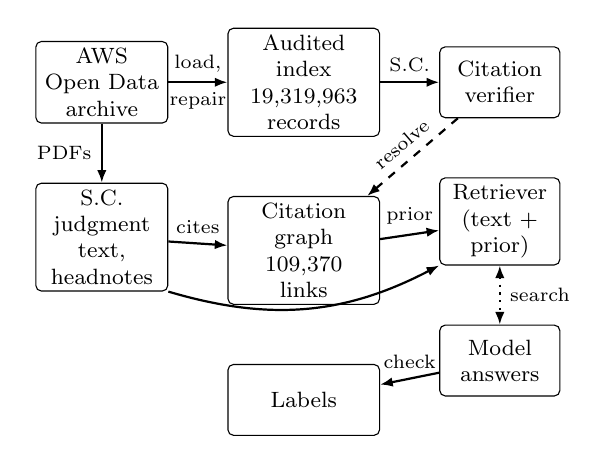
\begin{tikzpicture}[
  box/.style={draw, rounded corners=2pt, align=center, font=\footnotesize, minimum height=0.9cm, inner sep=2.5pt},
  arr/.style={-{Latex[length=1.6mm]}, thick},
  lbl/.style={font=\scriptsize, align=center}]
\node[box, text width=1.5cm] (aws) {AWS Open Data archive};
\node[box, text width=1.75cm, right=0.75cm of aws] (idx) {Audited index\\ \CorpusTotal{}\\ records};
\node[box, text width=1.35cm, right=0.75cm of idx] (ver) {Citation\\ verifier};
\node[box, text width=1.5cm, below=0.75cm of aws] (txt) {S.C. judgment text, headnotes};
\node[box, text width=1.75cm, below=0.75cm of idx] (graph) {Citation graph\\ \GraphEdges{}\\ links};
\node[box, text width=1.35cm, below=0.75cm of ver] (ret) {Retriever\\ (text + prior)};
\node[box, text width=1.35cm, below=0.75cm of ret] (llm) {Model\\ answers};
\node[box, text width=1.75cm, below=0.75cm of graph] (lab) {Labels};
\draw[arr] (aws) -- node[lbl, above] {load,} node[lbl, below] {repair} (idx);
\draw[arr] (idx) -- node[lbl, above] {S.C.} (ver);
\draw[arr] (aws) -- node[lbl, left] {PDFs} (txt);
\draw[arr] (txt) -- node[lbl, above] {cites} (graph);
\draw[arr, dashed] (ver) -- node[lbl, sloped, above] {resolve} (graph);
\draw[arr] (graph) -- node[lbl, above] {prior} (ret);
\draw[arr] (txt.south east) to[bend right=22] (ret.south west);
\draw[arr, {Latex[length=1.6mm]}-{Latex[length=1.6mm]}, dotted] (ret) -- node[lbl, right] {search} (llm);
\draw[arr] (llm) -- node[lbl, above] {check} (lab);
\end{tikzpicture}
\caption{Overview. The archive's metadata is loaded into an audited index; the verifier resolves citations and case names against its Supreme Court part. The text of every Supreme Court judgment yields headnotes and the citations each judgment makes, which the verifier resolves into a citation graph. The retriever searches headnotes by subject and ranks with the graph's citation counts. Model answers are checked by the verifier; in the search conditions the model queries the index or the retriever before answering.}
\label{fig:pipeline}
\end{figure}


\section{Related Work}
\textbf{Legal hallucination.} Dahl et al.\ found hallucination rates between 58\% (ChatGPT~4) and 88\% (Llama~2) on verifiable questions about United States federal cases \cite{dahl2024}, and Magesh et al.\ found that commercial retrieval-augmented legal research tools still hallucinate on 17--33\% of queries \cite{magesh2025}. Detector benchmarks \cite{liu2026checks}, LegalCiteBench \cite{legalcitebench} and a study of substituted cases and pinpoint pages \cite{verma2026} all concern United States law.

\textbf{Citation tools, networks and retrieval.} eyecite extracts and normalises United States citations \cite{eyecite} and CourtListener's lookup API flags invalid ones \cite{courtlistenerapi}; our verifier plays that role for the Supreme Court of India, whose neutral and S.C.R. formats and party-name conventions differ. Fowler et al.\ built the citation network of the United States Supreme Court \cite{fowler2007} and Minocha et al.\ one for Indian judgments that invoke Articles 264--300 \cite{minocha2015}. Prior-case retrieval takes its relevance judgments from the citations in the judgments themselves \cite{joshi2023ucreat,farber2020}, and retrieval-augmented generation grounds a model in retrieved documents \cite{lewis2020rag}. We build the citation network for the whole reported Supreme Court, use it both as a ranking signal and as relevance labels, and measure what retrieval changes in the authorities that models cite.

\textbf{Agents with citation checks.} Recent legal agents retrieve sources before answering and audit their citations: L-MARS \cite{lmars}, a retrieval system for Korean bar questions \cite{koreanrag}, Maat \cite{maat} and Parthenon, which wraps agents in deterministic checks for sources, dates and numbers \cite{parthenon}; a survey reviews the line \cite{liu2026survey}. Our checks can serve as such a layer for Indian law, and \S\ref{sec:system} uses them that way.

\textbf{Indian legal NLP and tools.} ILDC provides 35k Supreme Court judgments for judgment prediction \cite{ildc}, IL-TUR benchmarks Indian legal text understanding \cite{iltur} and NyayaRAG studies retrieval-augmented judgment prediction \cite{nyayarag}. The Supreme Court's own tools are assistive: SUVAS translates judgments and SUPACE extracts facts and precedents for judges \cite{suvas,supace}. Closest to our corpus, open-india-law releases text and embeddings for 12.8 million judgments from the same archive and treats a citation graph as out of scope \cite{openindialaw}. We add a documented audit of the archive's metadata, a verifier, an open citation graph of the Supreme Court, a benchmark of how models cite, and a workspace that puts these checks in an advocate's hands.

\section{An Open Index of Indian Judgments}
\label{sec:corpus}
\subsection{Source, audit and repair}
The AWS Open Data registry hosts two datasets published under CC-BY-4.0 by Dattam Labs: judgments of the Supreme Court from 1950 \cite{awssc} and of 25 High Courts \cite{awshc}, each with structured metadata in Parquet and the judgments as PDFs. We load only the metadata (no text and no PDFs) into one PostgreSQL 17 table, reading the Parquet files directly from S3. The result holds \CorpusTotal{} records: \CorpusSC{} Supreme Court judgments and \CorpusHC{} High Court judgments and orders (\CorpusCourts{} courts in all), with decision years from \CorpusYearMin{} to \CorpusYearMax. Each record stores a link to the original PDF in the archive, never the PDF itself.

High Court metadata reaches the archive through two paths. Records from the ``mobile'' path store only a bare file name where a bench-qualified path is needed, so the PDF link cannot be formed, a problem the archive's documentation notes without quantifying \cite{hcdatasetdoc}. Table~\ref{tab:mobile} does: \MobileTotal{} records in four High Courts (\MobilePct{} of the corpus) are affected, \MobileRecentPct{} of them decided in 2024--2026. The file name is not a usable identity either: \CollideStems{} file names occur in more than one bench of the same court, covering \CollideRows{} records, and in \CollideDiffBothPct{} of these the title and the decision date both differ. Keying on the file name, as our first load did, silently overwrites at least \CollideLost{} records; the case number (CNR) differs in all of them, so we key on it. We repair the mobile records by taking the bench from the S3 key of the metadata file and reconciling every record against a listing of the archive's actual PDF files, linking a record only when its file exists. This restores \MobileLinked{} links (\MobileLinkedPct). The remaining \MobileUnrecov{} records have no matching PDF in the archive, including all but \MPLinked{} of Madhya Pradesh's \MPMobile{} mobile records. After repair \LinkedPct{} of all records carry a link.

\begin{table}[t]
\caption{High Court records from the archive's mobile path, and the links restored by reconciliation against the archive's file listing.}
\label{tab:mobile}
\centering
\begin{tabular}{lrrr}
\toprule
High Court & Records & Mobile & Linked after repair \\
\midrule
Bombay & 2{,}446{,}330 & 643{,}216 & 537{,}441 (83.6\%) \\
Allahabad & 2{,}300{,}821 & 605{,}598 & 584{,}934 (96.6\%) \\
Madhya Pradesh & 693{,}219 & 42{,}695 & 5 ($<$0.1\%) \\
Himachal Pradesh & 292{,}894 & 7 & 7 (100.0\%) \\
\midrule
All four & 5{,}733{,}264 & 1{,}291{,}516 & 1{,}122{,}387 (86.9\%) \\
\bottomrule
\end{tabular}

\end{table}

\subsection{Validation and Supreme Court metadata}
We checked links against the live archive with HTTP HEAD requests. All \RecoveredChecked{} randomly sampled restored links resolve. For \UnresolvedChecked{} randomly sampled unrecoverable records the expected file does not exist in the decision-year folder or the two neighbouring years. All \NonmobileChecked{} sampled original links resolve, across \NonmobileCourts{} High Courts, as do all \SCLinksChecked{} sampled Supreme Court links.

Every one of the \CorpusSC{} Supreme Court judgments carries an S.C.R. citation (\SCSupp{}, \SCSuppPct, in a supplementary volume), and \SCwithNeutral{} carry a neutral citation, which the Court launched in 2023 \cite{scneutral}. Three properties matter for verification. The year field is the year of the S.C.R. volume, not of the decision, for \SCYearNe{} judgments (\SCYearNePct), so we use the decision date throughout. \SCDupGroups{} neutral citations are attached to more than one record (\SCDupRows{} records). And for each year from 1950 to 2013 except \INSCIncompleteList{} the index holds every neutral-citation number from 1 to the year's maximum, because the Court assigned them retrospectively to the judgments reported in the S.C.R. \cite{scneutral2}; a neutral citation missing from the index is therefore unassigned only for those \INSCCompleteCount{} years, while from 2014 the index, which holds reported judgments, contains between \INSCCovMin{} and \INSCCovMax{} of each year's numbers. A small HTTP service exposes keyword search, filters and exact lookups for CNR, neutral and S.C.R. citations (timings in \S\ref{sec:discussion}).

\section{Citation Verifier}
\label{sec:verifier}
The verifier takes a case name, a year and a citation string, as a model produced them, and decides whether they denote a real Supreme Court judgment in the index.

\textbf{Citations.} Neutral citations are parsed with the pattern \emph{year} \texttt{INSC} \emph{number}. S.C.R. citations are parsed in the bracketed official form and common variants such as \texttt{(1978) 2 SCR 621}, and a citation without a volume number (common for supplementary volumes) matches any volume of the same series, year and page. Citations to other law reports (SCC, AIR) cannot be resolved against the index and are left to the name match.

\textbf{Names.} A case name and a judgment's party names are split into words and initials, lower-cased, with stop-words (\emph{the}, \emph{v.}, \emph{ors.}) dropped and abbreviations expanded (\emph{C.B.I.}, \emph{U.P.}). Each word $t$ has weight $w(t)=\log(N/\mathrm{df}(t))$ over the $N$ Supreme Court judgments \cite{sparckjones}. Two words match if they are equal or, for words of five or more letters, if their similarity ratio \cite{difflib} is at least 0.85, which accepts transliteration variants such as \emph{Keshavananda}/\emph{Kesavananda} but not \emph{Patil}/\emph{Patel}. A rare given name may also match an initial in the judgment's title once a distinctive word has matched. With $M_a$ and $M_b$ the matched words of the name $a$ and of the judgment $b$, let $p=W(M_a)/W(a)$ and $r=W(M_b)/W(b)$, where $W$ sums word weights. The name score is the harmonic mean of $p$ and $r$, set to zero if $p<0.8$, so that an unmatched given name cannot be outweighed by common words such as \emph{State}. Candidates are judgments whose decision year or S.C.R. volume year lies within one year of the stated year.

\textbf{Labels.} With threshold $\tau=0.5$: \emph{VERIFIED} if some candidate's name score is at least $\tau$ and a neutral or S.C.R. citation, if given, points to that judgment or to one with matching parties; \emph{WRONG\_CITATION} if the parties match but the citation points elsewhere or nowhere; \emph{MISATTRIBUTED} if no candidate matches but the citation resolves to a different judgment; \emph{WRONG\_YEAR} if neither resolves but the name identifies exactly one judgment (or several orders in one matter) elsewhere in the corpus, with a score of at least 0.8 and a word found in at most 15 judgments, i.e.\ a real case cited with the wrong year; \emph{NOT\_FOUND} otherwise. VERIFIED establishes that a judgment with those parties exists near that year, not that it supports the proposition for which it was cited. We developed these rules on the T4 answers of three models, reviewing by hand a development sample of 56 decisions and every label that changed between versions, and then froze the verifier, recording hashes of its code, before running T5, scoring and drawing the held-out audit of \S\ref{sec:audit}.

\section{Judgment Text and Citation Graph}
\label{sec:graph}
\subsection{Text, extraction and resolution}
We downloaded the PDF of every Supreme Court judgment in the archive and extracted its text layer with PyMuPDF; the reports are scanned pages with an embedded OCR layer, so no further OCR is needed. \GraphTextOK{} of the \CorpusSC{} judgments were extracted (for \GraphTextFail{} the archive returned an error or an HTML page). Every judgment in the S.C.R. opens with the reporter's headnote, which we cut at the jurisdiction line (e.g.\ ``CIVIL APPELLATE JURISDICTION''), keep to at most 3{,}000 characters and clean of running heads and the margin letters A--H.

We find every reporter citation in the text (S.C.R., neutral, SCC and Supreme Court AIR citations) and resolve each distinct pair of citing judgment and citation in three tiers: \emph{number}, where an S.C.R. or neutral citation is looked up exactly in the index; \emph{parallel number}, where an SCC or AIR citation written directly beside an S.C.R. or neutral citation, as in \texttt{(2012) 1 SCC 40 : [2011] 13 SCR 309}, takes that number's judgment; and \emph{name}, where the case name written before the citation and the citation's year go through the frozen verifier and the pair is resolved only if exactly one judgment matches. If a number and the case name beside it point to different judgments, the pair is dropped. We developed the extractor on a pilot sample of \PilotN{} judgments and ran it once over the whole corpus; the manual check below uses only judgments outside the pilot.

\subsection{Size and accuracy}
\label{sec:graphres}
Across the \GraphTextOK{} judgments the extractor found \GraphUnits{} distinct pairs of a citing judgment and a reporter citation of another judgment. \GraphResolved{} of them (\GraphResolvedPct) were resolved: \GraphExact{} by number, \GraphParallel{} through a parallel number and \GraphName{} by case name and year; \GraphConflict{} pairs whose number and name disagreed were dropped. The resolved pairs form \GraphEdges{} distinct links between \GraphCiting{} citing and \GraphCited{} cited judgments, so \GraphCitedPct{} of the Supreme Court's reported judgments are cited by at least one later reported judgment. Resolution depends on the citing judgment's era (Table~\ref{tab:graph}): judgments cite mostly the S.C.R. until the 1980s, the commercial SCC from the 1990s, and parallel S.C.R. citations, which make resolution easy, only from the 2010s, so the 2000s are the hardest decade.

\begin{table}[t]
\caption{Citations of other reported judgments, by decade of the citing judgment, and how they were resolved.}
\label{tab:graph}
\centering
\footnotesize
\setlength{\tabcolsep}{4pt}
\begin{tabular}{lrrrrr}
\toprule
Citing & Citations & Resolved & \multicolumn{3}{c}{Resolved by} \\
\cmidrule(lr){4-6}
decade & & (\%) & Number & Parallel & Name \\
\midrule
1950s & 953 & 87.6 & 821 & 0 & 14 \\
1960s & 3{,}259 & 84.0 & 2{,}669 & 6 & 63 \\
1970s & 5{,}001 & 75.9 & 3{,}561 & 18 & 219 \\
1980s & 6{,}467 & 77.5 & 4{,}160 & 43 & 806 \\
1990s & 15{,}667 & 63.8 & 4{,}958 & 361 & 4{,}676 \\
2000s & 34{,}810 & 55.0 & 2{,}957 & 375 & 15{,}830 \\
2010s & 70{,}340 & 78.5 & 23{,}027 & 17{,}174 & 15{,}026 \\
2020s & 67{,}418 & 84.0 & 26{,}370 & 22{,}036 & 8{,}212 \\
\bottomrule
\end{tabular}

\end{table}

\textbf{Accuracy.} Where a citation carries an S.C.R. or neutral number and the case name beside it can also be resolved, the name and year alone reach the same record as the number in \GraphNameSamePct{} of \GraphNamePrecN{} cases; in another \GraphNameLoosePct{} they reach a different record with matching parties (for example another order in the same case), and in \GraphNameWrongPct{} a record with different parties. This is a label-free estimate of the precision of name-only links. Only \GraphLater{} links (\GraphLaterPct) point to a judgment decided after the citing one, which is impossible. We also checked by hand \GraphCheckN{} randomly drawn name-only links from judgments outside the pilot, against the citation context and the index record: all \GraphCheckOK{} were correct. Of \UnresN{} randomly drawn SCC and AIR citations that stayed unresolved, \UnresNotIndex{} cite judgments that are not in the index at all, because they were reported in the SCC or AIR but not in the S.C.R.; the other \UnresInIndex{} were lost to OCR errors or truncated names (\UnresExtraction), errors in the source (\UnresSource), names shared by several judgments (\UnresAmbig) and the frozen name parser (\UnresVerifier).

\textbf{Face validity.} The most cited judgments are \emph{Maneka Gandhi v.\ Union of India} (\GraphTopOneN{} citing judgments), \emph{Kesavananda Bharati} (\GraphTopTwoN) and \emph{Sharad Birdhi Chand Sarda v.\ State of Maharashtra} (\GraphTopThreeN), leading authorities on personal liberty, the basic structure and circumstantial evidence. Of the \GraphLandmarkN{} landmark judgments that we chose by hand for the benchmark before the graph existed, \GraphLandmarkCited{} are cited at least once, and their median in-degree is higher than that of \GraphLandmarkPct\% of all judgments.

\section{Finding Authorities by Subject}
\label{sec:retrieval}
\subsection{Retrievers and evaluation}
We index the title and headnote of every judgment in two ways. \emph{BM25} \cite{robertson2009} scores unigrams and bigrams. \emph{Dense} retrieval embeds each headnote with the open multilingual model bge-m3 \cite{chen2024m3}, run locally, and scores by cosine similarity with the embedded query. The \emph{hybrid} retriever takes the union of the top 300 judgments of each and adds their scores after normalising each to zero mean and unit variance over the candidates. A \emph{citation prior} adds the normalised $\log(1+c)$, where $c$ is the number of judgments in the graph that cite the candidate. We use the raw count; recursive measures such as PageRank \cite{page1999} are an alternative we did not test. Every combination is a weighted sum of these three scores, with weights chosen on a development split and never on the evaluation data.

The graph supplies relevance judgments without annotation: the judgments a decision cites are the authorities its bench considered, the standard setting of citation recommendation \cite{farber2020} and of Indian prior-case retrieval \cite{joshi2023ucreat}. For each held-out judgment that cites at least \RecMinTargets{} earlier judgments, the query is its headnote with every reporter citation, every ``X v.\ Y'' case name and every ``\ldots's case'' reference removed, so the query states the legal issues without naming the precedents; the targets are the judgments it cites. Only judgments decided before it are candidates, and the citation prior counts only citations made before it, so no information from the future is used. We choose weights on \RecNDev{} development judgments and report recall@10, recall@50, the share of queries with at least one target in the top 10 (hit@10) and mean reciprocal rank on \RecNTest{} other test judgments, with bootstrap 95\% intervals. We also score the \NumTopics{} T4 questions against their reference judgments.

\subsection{Results}
\label{sec:retres}
\RecPool{} judgments cite at least \RecMinTargets{} earlier judgments that the graph resolves. On the \RecNTest{} test judgments, which cite \RecMeanTargets{} of them on average, the hybrid retriever with the citation prior places \RecHybridPriorRTenPct{} of the cited judgments in its top 10, and at least one of them for \RecHybridPriorHitTen{} of the queries (Table~\ref{tab:recommend}). The prior helps every retriever: on the same queries it raises the recall@10 of the hybrid retriever by \RecDiffPrior{} (paired bootstrap 95\% CI \RecDiffPriorCI; better on \RecDiffPriorBetter{} queries, worse on \RecDiffPriorWorse), a relative gain of \RecPriorRelGain. Popularity alone is useless (\RecPopRTen): the prior only reorders judgments that already match the subject. The query scrubbing leaves some names behind: \RecLeakStrictPct{} of the cited judgments share a rare title word with the query, and scoring only the other targets changes little (\RecHybridPriorRTenUnleaked{} with the prior, \RecHybridRTenUnleaked{} without).

\begin{table}[t]
\caption{Citation recommendation on \RecNTest{} held-out judgments: given the headnote without citations and case names, retrieve the earlier judgments it cites. R@$k$ = share of cited judgments in the top $k$; Hit@10 = share of queries with at least one in the top 10; MRR = mean reciprocal rank of the first. Weights chosen on \RecNDev{} other judgments.}
\label{tab:recommend}
\centering
\footnotesize
\setlength{\tabcolsep}{4pt}
\begin{tabular}{lrrrr}
\toprule
Method & R@10 & R@50 & Hit@10 & MRR \\
\midrule
Most cited so far & 0.013 & 0.039 & 0.111 & 0.056 \\
BM25 & 0.151 & 0.321 & 0.662 & 0.390 \\
Dense (bge-m3) & 0.136 & 0.286 & 0.614 & 0.362 \\
BM25 + dense & 0.167 & 0.345 & 0.689 & 0.420 \\
BM25 + prior & 0.182 & 0.381 & 0.740 & 0.455 \\
Dense + prior & 0.159 & 0.323 & 0.686 & 0.426 \\
BM25 + dense + prior & 0.204 & 0.399 & 0.774 & 0.496 \\
\bottomrule
\end{tabular}

\end{table}

Searched with the question text, the hybrid retriever with the prior returns a judgment that decided the question among its top three results for \QHybridPriorHitThree{} of the \NumTopics{} questions, and among its top ten for \QHybridPriorHitTen{} (Table~\ref{tab:questions}); no model named such a judgment from memory for more than \RefClosedLlama{} questions. Every judgment the retriever returns exists, with its correct citations, by construction. The questions were written around landmark judgments, which are cited often, so this set favours the prior; the recommendation experiment has no such bias.

\begin{table}[t]
\caption{Retrieval for the \NumTopics{} T4 questions: questions whose top-$k$ results contain a reference judgment, and the share of reference judgments in the top 10 (R@10). Weights from the recommendation development split.}
\label{tab:questions}
\centering
\footnotesize
\setlength{\tabcolsep}{4pt}
\begin{tabular}{lrrrr}
\toprule
Retriever & Top 3 & Top 5 & Top 10 & R@10 \\
\midrule
Most cited & 2 & 2 & 2 & 0.04 \\
BM25 & 25 & 28 & 30 & 0.63 \\
Dense & 29 & 31 & 35 & 0.76 \\
BM25 + dense & 28 & 30 & 36 & 0.77 \\
BM25 + dense + prior & 33 & 35 & 37 & 0.84 \\
\bottomrule
\end{tabular}

\end{table}

\section{How Language Models Cite: Setup}
\label{sec:setup}
The benchmark uses \NumJudgments{} Supreme Court judgments: \NumLandmark{} landmark judgments that we identified by name and confirmed individually in the index, and \NumRandom{} judgments sampled at random (seeded) across eight periods from 1950 to 2023, all with a unique neutral citation whose year equals the decision year. There are five tasks. \textbf{T1} (\NumTOne{} items) asks for the judgment reported at an S.C.R. or neutral citation. \textbf{T2} (\NumTTwo{} items) asks the same for citations that cannot exist (30 neutral numbers above the last one issued in a year the index covers completely, and 30 S.C.R. citations to a volume at least three above the year's last), where declining is correct. \textbf{T3} (\NumTThree{} items) gives the parties and decision date and asks for the S.C.R. and neutral citations. \textbf{T4} (\NumTopics{} items) asks for up to three leading Supreme Court judgments on a legal question (e.g., whether the right to privacy is a fundamental right), each labelled by the verifier. \textbf{T5} gives the model the verifier's findings on its T4 answer and asks it to revise. For T4 we also record reference answers, the Supreme Court judgments that decided each question, one to four per question (\NumRefJudgments{} index records), including earlier decisions later overruled, such as \emph{Suresh Kumar Koushal} for Section~377. We compiled them after the closed-book runs and before the search runs and recorded their hash. A question counts as answered if a listed case matches a reference judgment under the verifier's rules, a lower bound on relevance.

We evaluate four open-weight models that run on an 8\,GB laptop GPU (NVIDIA RTX 4060) through Ollama \cite{ollama}, in 4-bit quantisation: Llama~3.1 8B \cite{llama3}, Qwen3 8B \cite{qwen3}, Gemma~3 4B \cite{gemma3} and Qwen2.5-VL 7B \cite{qwen25vl}. Every request uses the same system prompt (state only facts you are confident about, and say when you do not know), temperature~0, a fixed seed and a JSON schema for the output. Thinking is disabled for Qwen3; as an ablation we also run it with thinking on T1, T2 and T4.

In a \emph{name search} condition the models answer T1--T4 with two tools over the index metadata: \emph{search} returns the \SearchK{} judgments whose party names best match the query (ranked by the name score of \S\ref{sec:verifier}), and \emph{lookup} returns the judgment with a given neutral or S.C.R. citation, or reports that the index has none. The task prompt describes the tools, including that the index holds no subject matter. The model replies with one JSON action at a time and, after at most \SearchMaxActions{} actions, gives its final answer in the task's schema, scored like the closed-book answer; we use this protocol rather than native tool calling because Gemma~3 has none in Ollama. In two \emph{topic search} conditions we repeat T4 with the retriever of \S\ref{sec:retrieval} as the search tool, once without and once with the citation prior, and each result shows the parties, date, citations and the first 280 characters of the headnote. We tried the protocols on items outside the benchmark and froze the code and the reference answers by recording hashes before running each condition once. For T1 and T2 we report the share of items answered correctly, wrongly and declined; for T4 and T5 the share of cited cases in each verifier label and the number of questions whose list includes a reference judgment. Intervals are Wilson 95\% intervals \cite{wilson}; for T4 they treat cases as independent although cases cited for one question are related, so they understate the uncertainty.

\section{How Language Models Cite: Results}
\label{sec:results}
\textbf{Identifying and supplying citations (T1--T3).} Table~\ref{tab:t1t2} shows two opposite behaviours. Llama~3.1 and Gemma~3 answered almost every question and were almost always wrong. Llama identified \TOneCorrectLlama{} of the \TOneN{} real citations (\emph{Kesavananda Bharati}, by its S.C.R. citation); Gemma identified none. Both named a judgment for nearly every fabricated citation: \TTwoNamedLlama{} of 60 for Llama (\TTwoNamedPctLlama, 95\% CI \TTwoNamedCILlama) and \TTwoNamedGemma{} of 60 for Gemma (\TTwoNamedPctGemma, 95\% CI \TTwoNamedCIGemma). Their wrong answers were not near misses: the closest any came to the true judgment was a name score of \MaxWrongLenientLlama{} (Llama) and \MaxWrongLenientGemma{} (Gemma), well below 0.5. The two Qwen models took the opposite course and declined all 262 questions, which is correct for T2 but forfeits T1. With thinking disabled, no model identified more than \BestTOneCorrect{} of the \TOneN{} real citations. Given the parties and date and asked for the citations (T3), the models supplied \TThreeCorrectAll{} correct citations of \TThreeAskedAll{} requested; the Qwen models, which had declined every T1 question, now answered, and almost all were wrong. Of Qwen2.5-VL's neutral citations, \TThreeUnassignedQwenVL{} carry a number above the last one issued in a year the index covers completely, so they cannot exist (Table~\ref{tab:t3}).

\begin{table}[t]
\caption{Supplying the citations of \NumTThree{} known judgments, given parties and decision date. Corr.\ = exact match; Wrong = any other non-empty answer; Empty = no citation given.}
\label{tab:t3}
\centering
\setlength{\tabcolsep}{4pt}
\begin{tabular}{lrrrrrr}
\toprule
& \multicolumn{3}{c}{S.C.R. citation (\%)} & \multicolumn{3}{c}{Neutral citation (\%)} \\
\cmidrule(lr){2-4}\cmidrule(lr){5-7}
Model & Corr. & Wrong & Empty & Corr. & Wrong & Empty \\
\midrule
Llama 3.1 8B & 2.0 & 96.0 & 2.0 & 0.0 & 98.0 & 2.0 \\
Qwen3 8B & 0.0 & 83.2 & 16.8 & 1.0 & 80.2 & 18.8 \\
Qwen3 8B think & -- & -- & -- & -- & -- & -- \\
Gemma 3 4B & 0.0 & 100.0 & 0.0 & 0.0 & 100.0 & 0.0 \\
Qwen2.5-VL 7B & 0.0 & 11.9 & 88.1 & 0.0 & 90.1 & 9.9 \\
\bottomrule
\end{tabular}

\end{table}

\begin{table}[t]
\caption{Identifying a judgment from its citation. T1: \NumTOne{} real citations (\NumJudgments{} judgments, each by S.C.R. and neutral citation). T2: \NumTTwo{} citations that cannot exist. Corr.\ = named the right judgment; Named = named any judgment for a fabricated citation; Decl.\ = declined; Inv.\ = invalid output.}
\label{tab:t1t2}
\centering
\footnotesize
\setlength{\tabcolsep}{3pt}
\begin{tabular}{lrrrrrrr}
\toprule
& \multicolumn{4}{c}{T1: real citation (\%)} & \multicolumn{3}{c}{T2: fabricated (\%)} \\
\cmidrule(lr){2-5}\cmidrule(lr){6-8}
Model & Corr. & Wrong & Decl. & Inv. & Named & Decl. & Inv. \\
\midrule
Llama 3.1 8B & 0.5 & 99.0 & 0.0 & 0.5 & 98.3 & 0.0 & 1.7 \\
Qwen3 8B & 0.0 & 0.0 & 100.0 & 0.0 & 0.0 & 100.0 & 0.0 \\
Qwen3 8B think & 1.0 & 14.4 & 83.2 & 1.5 & 10.0 & 88.3 & 1.7 \\
Gemma 3 4B & 0.0 & 100.0 & 0.0 & 0.0 & 100.0 & 0.0 & 0.0 \\
Qwen2.5-VL 7B & 0.0 & 0.0 & 100.0 & 0.0 & 0.0 & 100.0 & 0.0 \\
\bottomrule
\end{tabular}

\end{table}

\textbf{Authorities for legal questions (T4).} Asked for up to three leading authorities on each of \NumTopics{} questions, the models named between \TFourCasesMin{} and \TFourCasesMax{} cases each (Table~\ref{tab:t4}). Only \TFourVerifiedRange{} of these could be matched to a Supreme Court judgment with the named parties within a year of the stated date; between \TFourNFMinPct{} (\TFourNFMinModel) and \TFourNFMaxPct{} (\TFourNFMaxModel) were NOT\_FOUND. The models cited almost exclusively the commercial SCC and AIR reports, which the index cannot resolve, so these labels rest on the party names and year. Only Qwen2.5-VL used the S.C.R. form to any extent, and all \TFourReporterResolvedMisQwenVL{} of those that resolved in the index pointed to a different judgment (MISATTRIBUTED): it attributed \texttt{1970 (2) SCR 1}, which is \emph{Sitabai v.\ Ram Chandra}, to an invented \emph{State of Maharashtra v.\ Keshav Bapuji Patil}.

\begin{table}[t]
\caption{T4: every case cited for \NumTopics{} legal questions, by verifier label. Ver.\ = VERIFIED (with Wilson 95\% interval), W.Yr.\ = WRONG\_YEAR, W.Cit.\ = WRONG\_CITATION, Misatt.\ = MISATTRIBUTED, N.F.\ = NOT\_FOUND.}
\label{tab:t4}
\centering
\footnotesize
\setlength{\tabcolsep}{3.5pt}
\begin{tabular}{lrrrrrrr}
\toprule
& & \multicolumn{6}{c}{Share of cited cases (\%)} \\
\cmidrule(lr){3-8}
Model & Cases & Ver. & 95\% CI & W.Yr. & W.Cit. & Misatt. & N.F. \\
\midrule
Llama 3.1 8B & 114 & 61.4 & 52--70 & 1.8 & 0.0 & 0.0 & 36.8 \\
Qwen3 8B & 117 & 50.4 & 42--59 & 7.7 & 0.0 & 0.0 & 41.9 \\
Qwen3 8B think & 94 & 35.1 & 26--45 & 4.3 & 0.0 & 0.0 & 60.6 \\
Gemma 3 4B & 117 & 23.9 & 17--32 & 6.8 & 0.0 & 0.0 & 69.2 \\
Qwen2.5-VL 7B & 102 & 22.5 & 16--32 & 0.0 & 0.0 & 11.8 & 65.7 \\
\bottomrule
\end{tabular}

\end{table}

\textbf{Verifier accuracy.}
\label{sec:audit}
We drew a fresh, stratified random sample of \AuditN{} T4 decisions from the four models, excluding every case on the development sheet, and judged each by hand against the index and our knowledge of the case law. The verifier was right in \AuditCorrect{} of \AuditN{} (\AuditPct). \AuditVerCorrect{} of \AuditVerN{} VERIFIED labels were correct (the error matched \emph{Narendra Kumar v.\ Union of India} to \emph{State Bank of India v.\ Narendra Kumar Pandey}), \AuditNFCorrect{} of \AuditNFN{} NOT\_FOUND labels were correct (both misses were real judgments whose titles contain OCR errors in the source), and all \AuditWYN{} WRONG\_YEAR and \AuditMisN{} MISATTRIBUTED labels were correct. Of the \AuditNFN{} audited NOT\_FOUND cases, \AuditNFFab{} named parties that match no Supreme Court judgment in any year, \AuditNFGeneric{} used names so common that same-named judgments exist only in other years, \AuditNFMisdated{} was a real judgment cited with a wrong year and an altered name, and \AuditNFNotJudgment{} was not a judgment at all.

\textbf{Feedback and reasoning.} For the \TFiveQAll{} T4 answers that contained an unverified case, we told the model what the check had found and asked it to revise its list. NOT\_FOUND cases fell from \TFiveNFBeforeAll{} to \TFiveNFAfterAll{} and the share of verified cases rose for every model, but the gain came entirely from removal: \TFiveRepeatedAll{} of the \TFiveCasesAfterAll{} cases in the revised lists were repeated from the first answers, only \TFiveNewCaseModels{} models named new cases (\TFiveNewCasesAll{} in all) and none could be verified, and the number of verified cases fell slightly, from \TFiveVerBeforeAll{} to \TFiveVerAfterAll. Feedback from an existence check makes an answer shorter and safer, not more complete (Table~\ref{tab:t5}).

\begin{table}[t]
\caption{T5: the T4 answers that contained an unverified case (Q), before and after the model revised them with the verifier's feedback.}
\label{tab:t5}
\centering
\footnotesize
\setlength{\tabcolsep}{3.5pt}
\begin{tabular}{lrrrrrrr}
\toprule
& & \multicolumn{2}{c}{Cases} & \multicolumn{2}{c}{Verified (\%)} & \multicolumn{2}{c}{Not found} \\
\cmidrule(lr){3-4}\cmidrule(lr){5-6}\cmidrule(lr){7-8}
Model & Q & Before & After & Before & After & Before & After \\
\midrule
Llama 3.1 8B & 30 & 87 & 48 & 49.4 & 87.5 & 42 & 4 \\
Qwen3 8B & 29 & 84 & 27 & 30.9 & 92.6 & 49 & 1 \\
Gemma 3 4B & 37 & 111 & 40 & 19.8 & 52.5 & 81 & 16 \\
Qwen2.5-VL 7B & 35 & 87 & 39 & 9.2 & 20.5 & 67 & 31 \\
\bottomrule
\end{tabular}

\end{table}

With thinking enabled Qwen3 wrote a median of \ThinkMedianChars{} characters of reasoning per item and took \ThinkMedianSec{}\,s instead of \NoThinkMedianSec{}\,s; it stopped declining but its extra answers were mostly wrong (it named a judgment for \ThinkTTwoNamed{} of the 60 fabricated citations), and on T4 its verified share fell from \NoThinkTFourVerPct{} to \ThinkTFourVerPct. At this scale, reasoning made the model more willing to answer without making it more accurate.

\textbf{Searching by name.} With access to the index the citation tasks became easy for most models: they identified between \SearchTOneCorrectMin{} and \SearchTOneCorrectMax{} of the \TOneN{} real citations, against at most \BestTOneCorrect{} without search. For legal questions the effect differs (Table~\ref{tab:t4conds}). Name search almost eliminated cases the index cannot find (NOT\_FOUND fell from \NFClosedAll{} to \NFSearchAll{} across the four models, and verified cases rose from \VerClosedAll{} to \VerSearchAll{}), but fewer answers contained a judgment that decided the question: \RefSearchAll{} of \RefQuestionsAll{} model--question pairs, against \RefClosedAll{} without search; counting each question once, \SignClosedNameWorse{} questions were answered by fewer models with name search and \SignClosedNameBetter{} by more (exact sign test, $p$~\SignClosedNameP). The cause is how the models searched. The tool description stated that the index holds no subject matter, yet Llama and Qwen2.5-VL mostly searched with the words of the question and listed the judgments whose party names happened to contain them. On whether ``procedure established by law'' must be fair, just and reasonable, Llama had cited \emph{Maneka Gandhi} without search; with search it listed \emph{Fair Air Engineers v.\ N.K.\ Modi} and \emph{Just Society v.\ Union of India}. These judgments exist, so the verifier labels them VERIFIED, yet none of the \SearchTopicCasesAll{} listed judgments that came only from such searches is a reference judgment.

\begin{table*}[t]
\caption{T4 under five conditions: from memory, after verifier feedback (T5 answers where revised, T4 otherwise), with name search over the index metadata, and with topic search over headnotes without and with the citation prior. Ref.\ = questions (of \NumTopics) whose list includes a judgment that decided the question; N.F.\ = listed cases the verifier could not find.}
\label{tab:t4conds}
\centering
\footnotesize
\setlength{\tabcolsep}{4pt}
\begin{tabular}{lrrrrrrrrrr}
\toprule
 & \multicolumn{2}{c}{From memory} & \multicolumn{2}{c}{After feedback} & \multicolumn{2}{c}{Name search} & \multicolumn{2}{c}{Topic search} & \multicolumn{2}{c}{Topic + prior} \\
\cmidrule(lr){2-3}\cmidrule(lr){4-5}\cmidrule(lr){6-7}\cmidrule(lr){8-9}\cmidrule(lr){10-11}
Model & Ref. & N.F. & Ref. & N.F. & Ref. & N.F. & Ref. & N.F. & Ref. & N.F. \\
\midrule
Llama 3.1 8B & 24 & 42 & 24 & 4 & 10 & 4 & 29 & 2 & 35 & 1 \\
Qwen3 8B & 13 & 49 & 13 & 1 & 12 & 1 & 24 & 0 & 33 & 0 \\
Gemma 3 4B & 8 & 81 & 8 & 16 & 5 & 1 & 27 & 0 & 32 & 0 \\
Qwen2.5-VL 7B & 3 & 67 & 3 & 31 & 0 & 2 & 29 & 0 & 33 & 0 \\
\midrule
All four & 48 & 239 & 48 & 52 & 27 & 8 & 109 & 2 & 133 & 1 \\
\bottomrule
\end{tabular}

\end{table*}

\textbf{Searching by subject.} Topic search changed the answers to the legal questions more than any other condition (Table~\ref{tab:t4conds}). Across the four models, answers contained a judgment that decided the question in \RefAllTopic{} of the \RefQuestionsAll{} pairs with topic search and in \RefAllTopicPrior{} with topic search and the citation prior, against \RefAllClosed{} from memory and \RefAllName{} with name search. Counting each question once, \SignClosedTopicPriorBetter{} questions were answered by more models with topic search and the prior and \SignClosedTopicPriorWorse{} by fewer (exact sign test, $p$~\SignClosedTopicPriorP). The prior's own contribution is smaller: adding it to topic search improved \SignTopicTopicPriorBetter{} questions and worsened \SignTopicTopicPriorWorse{} ($p$~\SignTopicTopicPriorP). The gain was largest for the model that knew least: Qwen2.5-VL named a reference judgment for \RefClosedQwenVL{} questions from memory and for \RefTopicPriorQwenVL{} with topic search and the prior. At the same time almost every listed case was verified: \VerPctAllTopicPrior{} of the \CasesAllTopicPrior{} cases listed with topic search and the prior are VERIFIED and \NFAllTopicPrior{} is NOT\_FOUND, against \VerPctAllClosed{} and \NFAllClosed{} from memory. The models listed mostly judgments that the search had shown them. On workplace sexual harassment, Qwen2.5-VL named a non-existent \emph{Sukanya v.\ Union of India} from memory; with topic search it listed \emph{Medha Kotwal Lele v.\ Union of India}, and with the prior it listed \emph{Vishaka}.

\section{VakilBuddy: A Citation-Grounded Workspace}
\label{sec:system}
VakilBuddy is a prototype litigation workspace for advocates. It is a web application organised around a \emph{matter} (a case file) whose tabs cover research, evidence, arguments, drafting, hearing preparation and case status. A matter's data stays in the user's browser; a small server serves the page and calls the model provider, and a separate service over the index answers searches and lookups. Four properties follow from the findings above.

\textbf{The index is the source of truth for authorities.} Search over the index (exact lookup by CNR, neutral or S.C.R. citation, full-text and typo-tolerant search, filters by court, year and outcome) sits in the matter's research tab, where an advocate pins the judgments the matter relies on, each with a note of what it is relied on for. A citation check finds the citations and case names in a draft or in pasted text with patterns, looks each one up in the index, and reports whether the case exists, whether the number belongs to another case, whether the number is wrong, whether nothing is found, or whether it is a High Court case that cannot be checked (\S\ref{sec:case}). This check is simpler than the verifier of \S\ref{sec:verifier}: it expands state abbreviations and tolerates a one-letter spelling slip, but it searches the index by whole words, so a title that the archive spells differently is not found by name. Like the verifier it confirms existence, not that a judgment supports the proposition.

\textbf{Model text is bounded by sources.} Model requests go to OpenRouter \cite{openrouter} or any OpenAI-compatible endpoint; the key is kept on the server and never returned to the browser. A draft written by the model may cite only the authorities pinned to the matter and list only the matter's own documents as annexures, leaves a visible blank where a fact is missing, and has its citations checked in the same response. Every model answer carries the model's name, and where an action names cases they are looked up in the index and marked. For the actions that read the advocate's own documents, an answer is kept only if the documents support it: a position attributed to a witness is kept only if its content words, and every date and number in it, appear in that witness's statement; a next hearing date is kept only if the order writes it; and a chronology's source, and the document a witness is to be confronted with, must be documents that were supplied, with a dated event kept only if the documents write its date. Items that fail are dropped and counted. A failed model call is shown as an error and never replaced by a canned answer, and the percentages a model may offer for risk are not used.

\textbf{Evidence is read where it lies.} Text, Word and PDF files with a text layer are read directly, with pdf.js \cite{pdfjs}; scanned pages and photographs are read by Tesseract \cite{smith2007} in English, Hindi and Marathi inside the browser, so the files are never uploaded and only the text is kept. The text is searched across a matter's documents. Dates and rupee amounts, including Devanagari digits, are found by pattern together with the nearest event word, and two documents that give different dates or amounts beside the same word are listed as possible inconsistencies: places to look, never findings.

\textbf{Dates and drafts follow rules the advocate can inspect.} A limitation calculator holds \CasePeriods{} periods, each naming its source (the Limitation Act, 1963 \cite{limitationact}, the Supreme Court Rules, 2013 \cite{scrules}, the Code of Civil Procedure and others). It leaves out the day of the event (s.~12(1)) and, where the law allows it, the time taken to obtain a certified copy (s.~12(2)), runs a period that ends on a closed day to the day the court reopens (s.~4), and shows how each date was counted. Drafting offers \CaseFormats{} built-in formats, keeps the last twelve versions of a draft with a word-level redline between any two, takes reviewers' comments, and exports a Word file only after the advocate approves. The workspace files and sends nothing; a WhatsApp reminder opens with its text written and the advocate presses Send.

\textbf{Status.} The workspace is covered by \CaseTestsWorkspace{} automated tests and its index service by \CaseTestsApi{}. Model calls have been tested against a stub provider and a local open-weight model; hosted models, including those reached through OpenRouter, are untested. Apart from the matter of \S\ref{sec:case}, the matters in the workspace are sample data, and there is no user study.


\section{A Worked Case}
\label{sec:case}
We ran the workspace on a real Supreme Court case, \emph{Rajendra S/o Ramdas Kolhe v.\ State of Maharashtra} (Criminal Appeal No.~2281 of 2011, decided 15 May 2024, 2024~INSC~422), a murder appeal that turns on a dying declaration; the Court dismissed it. The judgment, the Court's own summaries of the six prosecution witnesses, the orders it recites and a short draft written for this test are in \texttt{sample-case/}, and the scripts that produce every number below are in \texttt{paper/final/case\_study/}.

\textbf{Reading the record.} The Evidence tab read the judgment (\CaseJudgWords{} words) and found \CaseJudgDates{} dates and \CaseJudgAmounts{} amount. A search for ``Ex.~59'', the deceased's written dying declaration, finds \CaseJudgExhibit{} places in the judgment and \CaseStmtExhibit{} in the witness summaries (\CaseStmtWords{} words, \CaseStmtDates{} dates). The recited orders (\CaseOrdersWords{} words, \CaseOrdersDates{} dates) give no date or amount that differs from the other documents beside the same event word, so the list of possible inconsistencies is empty (\CaseInconsistencies).

\textbf{Checking a draft.} The draft is a few paragraphs of submissions on the dying declaration, into which we planted errors (Table~\ref{tab:case}). The citation check found \CaseCiteFound{} cases. Of these, \CaseCiteVerified{} were confirmed. One has the right parties and a wrong volume (\emph{Paniben}, cited as [1992] 9 S.C.R.\ 197 and reported at [1992] 2 S.C.R.\ 197). One gives the appellant's own case the number of \emph{Khushal Rao v.\ State of Bombay}, and the check reports that the number belongs to another case. One, \emph{Verma v.\ State of Karnataka}, does not exist and was not found. One is a High Court case, which the check reports as not checkable. We planted the errors, so this shows that the check catches those kinds of error, not how often they occur.

\begin{table}[t]
\caption{The draft with planted errors and what the workspace's citation check reported.}
\label{tab:case}
\centering
\footnotesize
\setlength{\tabcolsep}{3pt}
% GENERATED by case_study/make_case_tex.mjs. Do not edit.
\begin{tabular}{@{}>{\raggedright\arraybackslash}p{1.3in}>{\raggedright\arraybackslash}p{0.95in}>{\raggedright\arraybackslash}p{0.85in}@{}}
\toprule
Case as cited & Citation & Verdict \\
\midrule
Khushal Rao v. State of Bombay & [1958] 1 S.C.R. 552 \textperiodcentered{} 1957 INSC 79 & Confirmed \\
Ashabai v. State of Maharashtra & [2013] 1 S.C.R. 115 & Confirmed \\
Lakhan v. State of Madhya Pradesh & [2010] 9 S.C.R. 705 \textperiodcentered{} 2010 INSC 489 & Confirmed \\
Paniben (Smt.) v. State of Gujarat & [1992] 9 S.C.R. 197 & Wrong number \\
Sher Singh v. State of Punjab & 2008 INSC 204 & Confirmed \\
Rajendra Kolhe v. State of Maharashtra & [1958] 1 S.C.R. 552 & Number of another case \\
Verma v. State of Karnataka & [2011] 5 S.C.R. 410 & Not found \\
State v. Rao & (name only) & High Court, not checkable \\
\bottomrule
\end{tabular}

\end{table}

The case also exposed three defects in how the workspace's own check searches the index: a state written in full where the archive writes ``M.P.'', a party name matched to a different case, and a spelling slip in a title. We fixed them and added regression tests. One limit remains: \emph{Sudhakar v.\ State of Madhya Pradesh}, which the archive spells ``Shudhakar'', is found by its S.C.R.\ number but not by name, because the index is searched by whole words.

\textbf{Dates.} A review petition in the Supreme Court lies within 30 days of the judgment (Order~XLVII Rule~2, Supreme Court Rules, 2013 \cite{scrules}). Given \CaseLimitStart, the limitation calculator returns \CaseLimitDate{} and shows that the day of the judgment is left out of the count.

\textbf{Checks on model text.} We sent the real prompts of three model actions that read these documents to \GroundModel{}, one of the four models of \S\ref{sec:setup}, three times each (temperature 0.2, seeds 1--3, a context of 8{,}192 tokens), kept the model's raw answer, and counted what the checks of \S\ref{sec:system} removed (Table~\ref{tab:ground}).

\begin{table}[t]
\caption{What the source checks removed from \GroundModel's answers on the worked case, \GroundRuns{} runs per action.}
\label{tab:ground}
\centering
\footnotesize
\setlength{\tabcolsep}{3pt}
% Every number is a macro from numbers_case.tex (generated), so this table cannot disagree with the runs.
\begin{tabular}{@{}>{\raggedright\arraybackslash}p{0.95in}>{\raggedright\arraybackslash}p{0.85in}>{\raggedright\arraybackslash}p{0.5in}>{\raggedright\arraybackslash}p{1.0in}@{}}
\toprule
Action & Model gave & Removed & Removed because \\
\midrule
Compare witness statements & \GroundMatrixProposed{} points & \GroundMatrixDropped{} & a position not in that witness's statement \\
Digest an order & \GroundDigestRuns{} next dates & \GroundDigestInvented{} & the order does not write the date \\
Chronology from documents & \GroundTimelineProposed{} dated events & \GroundTimelineDropped{} & a date not in the documents \\
 & \GroundSourcesNamed{} sources & \GroundSourcesInvented{} & not a supplied document \\
 & \GroundQDocsNamed{} documents to confront a witness with & \GroundQDocsInvented{} & not a supplied document \\
\bottomrule
\end{tabular}

\end{table}

The witness comparison returned \GroundMatrixProposed{} points over \GroundMatrixRuns{} runs (\GroundMatrixEmptyRuns{} run returned none). The check dropped \GroundMatrixDropped, a point whose second side named no witness, and kept \GroundMatrixKept, which quote the statements faithfully. The check tests fidelity to the source, not whether two statements conflict, and whether a kept point is a contradiction an advocate could use is a legal judgment we do not make. In all \GroundDigestRuns{} runs the order digest gave a next hearing date, \GroundDigestDates, worked out from ``two weeks from today''; the order writes none, and the check replaced each with ``not stated in the order''. The chronology proposed \GroundTimelineProposed{} dated events; \GroundIsoMissing{} of \GroundIsoProposed{} dates were not in the documents, and their events were dropped. The model named \GroundSourcesNamed{} sources and \GroundQDocsNamed{} documents to confront a witness with, and \GroundSuppliedClause. We needed a context of 8{,}192 tokens: at Ollama's default of 4{,}096 the chronology prompt, of about 4{,}000 tokens, left room for only 100 tokens of answer. This is one case, one small model and three runs per action. It shows that the checks remove what the documents do not support, not how often a larger or hosted model would produce it.


\section{Discussion}
\label{sec:discussion}
\textbf{Existence and authority are different checks.} A verifier over an index of names and citations catches fabricated cases, and feedback from it or search over it removed almost all of them. It did not help the models find the judgment that decides a question, and name search made that rarer, because the models searched with the question's words and listed any judgment whose parties happened to share them. A real but irrelevant judgment passes an existence check, so a system that shows only ``verified'' citations can look more reliable while citing worse authorities. Finding the authority needs what the metadata lacks: a description of what each judgment decided, which the reporter's headnote supplies, and a record of which judgments the Court itself relies on, which the citation graph supplies.

\textbf{The retriever does the work.} Listing the retriever's top three results answers about as many questions as the models that use it (\QHybridPriorHitThree{} against \RefTopicPriorGemma--\RefTopicPriorLlama), and the models listed almost only what the search had shown them. For a system that must not invent authorities this is the desirable division of labour: the index guarantees existence, the retriever and the graph supply relevance, and the model at most phrases and orders the result. The prior encodes the Court's own judgment of importance, as network measures of precedent do for the United States Supreme Court \cite{fowler2007}, but it favours old and frequently cited judgments, including judgments later overruled such as \emph{A.D.M.\ Jabalpur}, which a lawyer must cite as overruled.

\textbf{Declining one question is not reliability, and neutral citations invite invention.} The two Qwen models declined every request to identify a judgment from its citation, which looks like calibrated caution, yet asked for the citation of a judgment they had just been told exists they produced one for most judgments, nearly all wrong. The Supreme Court assigned neutral citations retrospectively to its reported judgments from 1950 \cite{scneutral,scneutral2}, so a model is unlikely to have seen them in use, yet it produced them readily. The same property makes them easy to check: for the \INSCCompleteCount{} years whose numbering the index holds completely, a single lookup settles whether a neutral citation exists.

\textbf{What remains unchecked.} Neither the verifier nor the retriever checks that a judgment supports the proposition it is cited for, which needs the judgment's reasoning and is hard even for strong models \cite{verma2026}; the graph records that one judgment cites another, not whether it follows, distinguishes or overrules it. Citations to the SCC and AIR reports are resolved through parallel S.C.R. citations or by party names, never by their own numbers. The graph and the verifier cover the Supreme Court only: the High Court records in the index have no citation fields (none of \HCMetaN{} sampled records had one), so extracting their citations needs the judgments themselves, \HCRecords{} PDFs of about \HCTotalTB\,TB in all by our sample (95\% interval \HCTotalTBLow--\HCTotalTBHigh\,TB), which we did not download.

\textbf{Limitations.} We evaluated four open-weight models of roughly 4 to 8 billion parameters in 4-bit quantisation, with one prompt and greedy decoding; larger and hosted models may know many more landmark citations and may balance answering and declining differently. We have not benchmarked the hosted models that VakilBuddy calls. The benchmark is small (\NumJudgments{} judgments, \NumTopics{} questions) and the landmark set is our own selection. The audit labels, the reference answers and the manual check of the graph come from a single annotator, working from the index, the judgment text and published sources, so we cannot report inter-annotator agreement. The reference answers were compiled after the closed-book runs, measure relevance only from below and, being landmarks, favour the citation prior; the recommendation experiment has neither problem but treats the judgments a decision cites as its only relevant authorities. The frozen name parser misreads a name that ends in ``v.''\ with no respondent. The corpus is a snapshot with its own errors: titles contain OCR errors, some judgments are filed under the wrong year, and \GraphTextFail{} PDFs are missing. VakilBuddy is a prototype: apart from the worked case its matters are sample data, its citation check is simpler than the evaluated verifier, the evaluated verifier and retriever are research code not yet connected to it, and we ran no user study, so we make no claim about drafting quality or time saved.

\textbf{Serving cost.} Everything runs on one laptop with default PostgreSQL settings. We timed \LatQueries{} queries to the index over HTTP, each run twice, directly after a database restart: exact lookups by CNR, neutral or S.C.R. citation took a median of \LatExactMedian{}\,ms, and keyword queries for common phrases a median of \LatCommonFirstMedian{}\,ms on first touch and \LatCommonWarmMedian{}\,ms when repeated. The verifier checked a cited case in a median of \VerifyMedianMs{}\,ms (95th percentile \VerifyPNinetyFiveMs{}\,ms), and a retrieval query, including embedding the query, took about \QueryMs{}\,ms on average.

\section{Conclusion}
\label{sec:conclusion}
Indian courts now treat reliance on fabricated precedents as misconduct \cite{gummadi}, so a model-drafted citation must be checked before it reaches a court. We built the checks from open data: an audited index of \CorpusTotal{} judgments and orders, a verifier for Supreme Court citations whose labels were correct in \AuditPct{} of a held-out audit, and an open citation graph of \GraphEdges{} links extracted from the text of every reported Supreme Court judgment, whose name-only links reach the same record as the citation number in \GraphNameSamePct{} of checkable cases. Small open models answering from memory fabricate freely. An existence check, as feedback or as a search tool, removes the fabricated cases but not the lack of authority. Search by subject over the reporters' headnotes, ranked with the citation counts of the graph, finds the judgments that decide a question: its top three results do so for \QHybridPriorHitThree{} of \NumTopics{} questions, and with it the same models named such a judgment in \RefAllTopicPrior{} of \RefQuestionsAll{} cases while \VerPctAllTopicPrior{} of the cases they listed were verified. VakilBuddy puts the index, a citation check and checks on model-written text in an advocate's workspace, and a worked Supreme Court case shows them catching planted citation errors and unsupported model output. Checking existence is cheap and should run before any citation reaches a court. Finding authority needs text and the citation network. Checking that a judgment supports what it is cited for remains open, as does connecting the evaluated retriever to the workspace and measuring what it saves an advocate.

\section*{Acknowledgment}
An AI assistant (Claude, Anthropic) was used to write the software, run the experiments and analyses, produce the first-pass labels of the verifier audit, the manual check of the citation graph and the reference answers for T4, and draft the text. The authors are responsible for the content.

\section*{Data and Code Availability}
The index builder, repair scripts, verifier, citation extractor, citation graph (every resolved and unresolved citation with its resolution tier), headnote embeddings, retrieval code, benchmark items, prompts, raw model outputs, scoring code, the workspace and the worked-case scripts and files are available from the authors. The underlying data are CC-BY-4.0 \cite{awssc,awshc}.

\bibliographystyle{IEEEtran}
\bibliography{refs,refs_extra}

\end{document}
